\documentclass[UTF8,table,fontset=adobe]{ctexbeamer}
% \documentclass[UTF8,table]{beamer}
% \usepackage[fontset=adobe]{ctex}

\mode<presentation>
{
  \usetheme{Madrid}
}
\setbeamercolor{bgcolor}{fg=yellow,bg=cyan}
% 使所有隐藏的文本完全透明、动态,而且动态的范围很小
\beamertemplatetransparentcovereddynamic
% 使itemize环境中变成小球,这是一种视觉效果
\beamertemplateballitem
% 为所有已编号的部分设置一个章节目录,并且编号显示成小球
\beamertemplatenumberedballsectiontoc
% 将每一页的要素的要素名设成加粗字体
\beamertemplateboldpartpage
% item逐步显示时,使已经出现的item、正在显示的item、将要出现的item呈现不同颜色
\def\hilite<#1>{
 \temporal<#1>{\color{gray}}{\color{blue}}
    {\color{blue!25}}
}

% 设定英文字体
% \usepackage[no-math]{fontspec}
\setmainfont{Times New Roman}
\setsansfont{Arial}
\setmonofont{Courier New}
% % 设定中文字体
% \usepackage[BoldFont,SlantFont,CJKchecksingle,CJKnumber]{xeCJK}
% \setCJKmainfont[BoldFont={Adobe Heiti Std},ItalicFont={Adobe Kaiti Std}]{WenQuanYi Micro Hei}
% \setCJKsansfont{Adobe Heiti Std}
% \setCJKmonofont{Adobe Fangsong Std}
% \punctstyle{hangmobanjiao}
% \defaultfontfeatures{Mapping=tex-text}
% \usepackage{xunicode}
% \usepackage{xltxtra}
% \XeTeXlinebreaklocale "zh"
% \XeTeXlinebreakskip = 0pt plus 1pt minus 0.1pt

\renewcommand{\today}{\number\year 年 \number\month 月 \number\day 日}

\usepackage{hyperref}
\hypersetup{xetex,bookmarksnumbered=true,bookmarksopen=true,pdfborder=1,breaklinks,colorlinks,linkcolor=cyan,filecolor=black,urlcolor=blue,citecolor=green}

%分栏
\usepackage{multicol}

% 插入图片
\usepackage{graphicx}
\graphicspath{{figures/}}
% 图文混排
% \usepackage{floatflt}

% 可能用到的包
% \usepackage{amsmath,amssymb}
% \usepackage{setspace}
% \usepackage{colortbl,xcolor}

%五角星
% \usepackage{MnSymbol}

%去除图表标题中的figure等
\usepackage{caption}
\captionsetup{labelformat=empty,labelsep=none}

\usepackage{tabu}
%表格自动换行
\usepackage{tabularx} 
\usepackage{multirow}

%罗马数字
\makeatletter
\newcommand{\rmnum}[1]{\romannumeral #1}
\newcommand{\Rmnum}[1]{\expandafter\@slowromancap\romannumeral #1@}
\makeatother

%插入源代码
\usepackage{listings}
\lstset{
  language=bash,                  % 程序语言名称:TeX, Perl, R, sh, bash, Awk
  basicstyle=\normalsize\tt,      %\tt指monospace字体族,程序源代码使用此族字体表示更加美观
  numbers=left,                   % 行号位置(左侧)
  numberstyle=\small,             % 行号字体的字号
  stepnumber=1,                   % 行号的显示步长
  numbersep=5pt,                  % 行号与代码间距
  backgroundcolor=\color{white},  % 背景色;需要 \usepackage{color}
  showspaces=false,               % 不显示空格
  showstringspaces=false,         % 不显示代码字符串中的空格标记
  showtabs=false,                 % 不显示 TAB
  tabsize=4, 
  frame=shadowbox,                % 把代码用带有阴影的框圈起来
  captionpos=b,                   % 标题位置
  breaklines=true,                % 对过长的代码自动断行
  breakatwhitespace=false,        % 断行只在空格处
  extendedchars=false,            % 解决代码跨页时,章节标题,页眉等汉字不显示的问题
  %escapeinside={\%*}{*},         % 跳脱字符,添加注释,暂时离开 listings 
  %escapeinside=``,
  commentstyle=\color{red!50!green!50!blue!50}\tt,  %浅灰色的注释
  rulesepcolor=\color{red!20!green!20!blue!20},     %代码块边框为淡青色
  keywordstyle=\color{blue!70}\bfseries\tt,         %代码关键字的颜色为蓝色,粗体
  identifierstyle=\tt,
  stringstyle=\tt,                % 代码字符串的特殊格式
  keepspaces=true,
  breakindent=1em,
  %breakindent=22pt,
  %breakindent=4em,
  breakautoindent=true,
  flexiblecolumns=true,
  aboveskip=1em,                  %代码块边框
  xleftmargin=2em,
  xrightmargin=2em
}


\begin{document}

%\includeonlyframes{current}

\logo{
\includegraphics[height=0.08\textwidth]{tijmu.png}}

% 在每个Section前都会加入的Frame
\AtBeginSection[]
{
  \begin{frame}<beamer>
    %\frametitle{Outline}
    \frametitle{教学提纲}
    \setcounter{tocdepth}{3}
    \begin{multicols}{2}
      \tableofcontents[currentsection,currentsubsection]
      %\tableofcontents[currentsection]
    \end{multicols}
  \end{frame}
}
% 在每个Subsection前都会加入的Frame
\AtBeginSubsection[]
{
  \begin{frame}<beamer>
%%\begin{frame}<handout:0>
%% handout:0 表示只在手稿中出现
    \frametitle{教学提纲}
    \setcounter{tocdepth}{3}
    \begin{multicols}{2}
    \tableofcontents[currentsection,currentsubsection]
    \end{multicols}
%% 显示在目录中加亮的当前章节
  \end{frame}
}

\begin{frame}[plain]
  \begin{center}
    {\Huge 系统生物学\\}
    \vspace{1cm}
    {\LARGE 天津医科大学\\}
    %\vspace{0.2cm}
    {\LARGE 生物医学工程与技术学院\\}
    \vspace{1cm}
    {\large 2016-2017学年上学期(秋)\\ 2013级生信班}
  \end{center}
\end{frame}



% \includeonlyframes{current}

\title[概论]{第一章\quad 系统生物学概论}
\author[Yixf]{伊现富(Yi Xianfu)}
\institute[TIJMU]{天津医科大学(TIJMU)\\ 生物医学工程与技术学院}
\date{2016年9月}

%\begin{frame}
\end{frame}

\begin{frame}
  \frametitle{授课教材}
  \begin{figure}
    \centering
    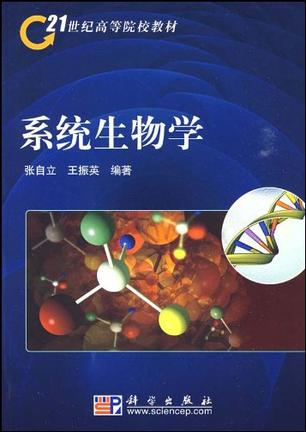
\includegraphics[width=5cm]{c0.book.jpg}
  \end{figure}
\end{frame}

\begin{frame}
  \frametitle{课程安排 | 理论课}
  \begin{table}
    \centering
    \rowcolors[]{1}{blue!20}{blue!10}
    \begin{tabular}{cllcc}
      \hline
      \rowcolor{blue!50}顺序 & 授课内容 & 教材章节 & 学时 & 授课教师\\
      \hline
      1 & 概论 & 第1章 & 2 & 伊现富\\
      2 & 基因组学 & 第2章 & 6 & 伊现富\\
      3 & 转录组学 & 第3章 & 6 & 伊现富\\
      4 &  & 第4章 & 2 & \\
      5 &  & 第5章 & 2 & \\
      6 &  & 第6章 & 2 & \\
      7 &  & 第7章 & 2 & \\
      8 &  & 第8章 & 2 & \\
      9 &  & 第9章 & 2 & \\
      \hline
    \end{tabular}
  \end{table}
\end{frame}

\begin{frame}
  \frametitle{课程安排 | 实验课}
  \begin{table}
    \centering
    \rowcolors[]{1}{blue!20}{blue!10}
    \begin{tabular}{cllcc}
      \hline
      \rowcolor{blue!50}顺序 & 实验内容 & 理论知识 & 学时 & 授课教师\\
      1 & 测序数据质控与预处理 & 基因组 & 3 & 伊现富\\
      2 & 外显子组测序数据分析 & 基因组 & 3 & 伊现富\\
      3 & 转录组测序数据分析 & 转录组 & 3 & 伊现富\\
      4 & & & 3 & \\
      5 & & & 3 & \\
      6 & & & 3 & \\
      \hline
    \end{tabular}
  \end{table}
\end{frame}

\begin{frame}
  \frametitle{考核方式}
  \begin{enumerate}
    \item 理论课:50\%
      \begin{enumerate}
        \item 平时表现:10\%
        \item 闭卷考试:40\%
      \end{enumerate}
    \item 实验课:30\%
      \begin{enumerate}
        \item 平时表现:10\%
        \item 实验报告:20\%
      \end{enumerate}
    \item 课堂讨论:20\%
      \begin{enumerate}
        \item 报告答辩:10\%
        \item 报告论文:10\%
      \end{enumerate}
  \end{enumerate}
\end{frame}



\begin{frame}
  \titlepage
\end{frame}

\begin{frame}[plain]
  \frametitle{教学提纲}
  \setcounter{tocdepth}{3}
  \begin{multicols}{2}
    \tableofcontents
  \end{multicols}
\end{frame}


\section{咬文嚼字}
\subsection{组分拆分}
\begin{frame}
  \frametitle{概论 | 咬文嚼字 | 系统生物学}
  \begin{huge}
  \begin{center}
  系统生物学 \\ = \\ 系统 \\ + \\ 生物 \\ + \\ 科学   
\end{center}
  \end{huge}
\end{frame}

\subsection{组分分析}
\begin{frame}[t]
  \frametitle{概论 | 咬文嚼字 | 系统}
  \begin{block}{系统}
    系统(system)泛指由一群有关联的个体组成,根据某种规则运作,能完成个别元件不能单独完成的工作的群体。\\
    古希腊语原意:“总体”,“整体”或“联盟”
  \end{block}
  \pause
  \begin{figure}
    \centering
    \only<2->{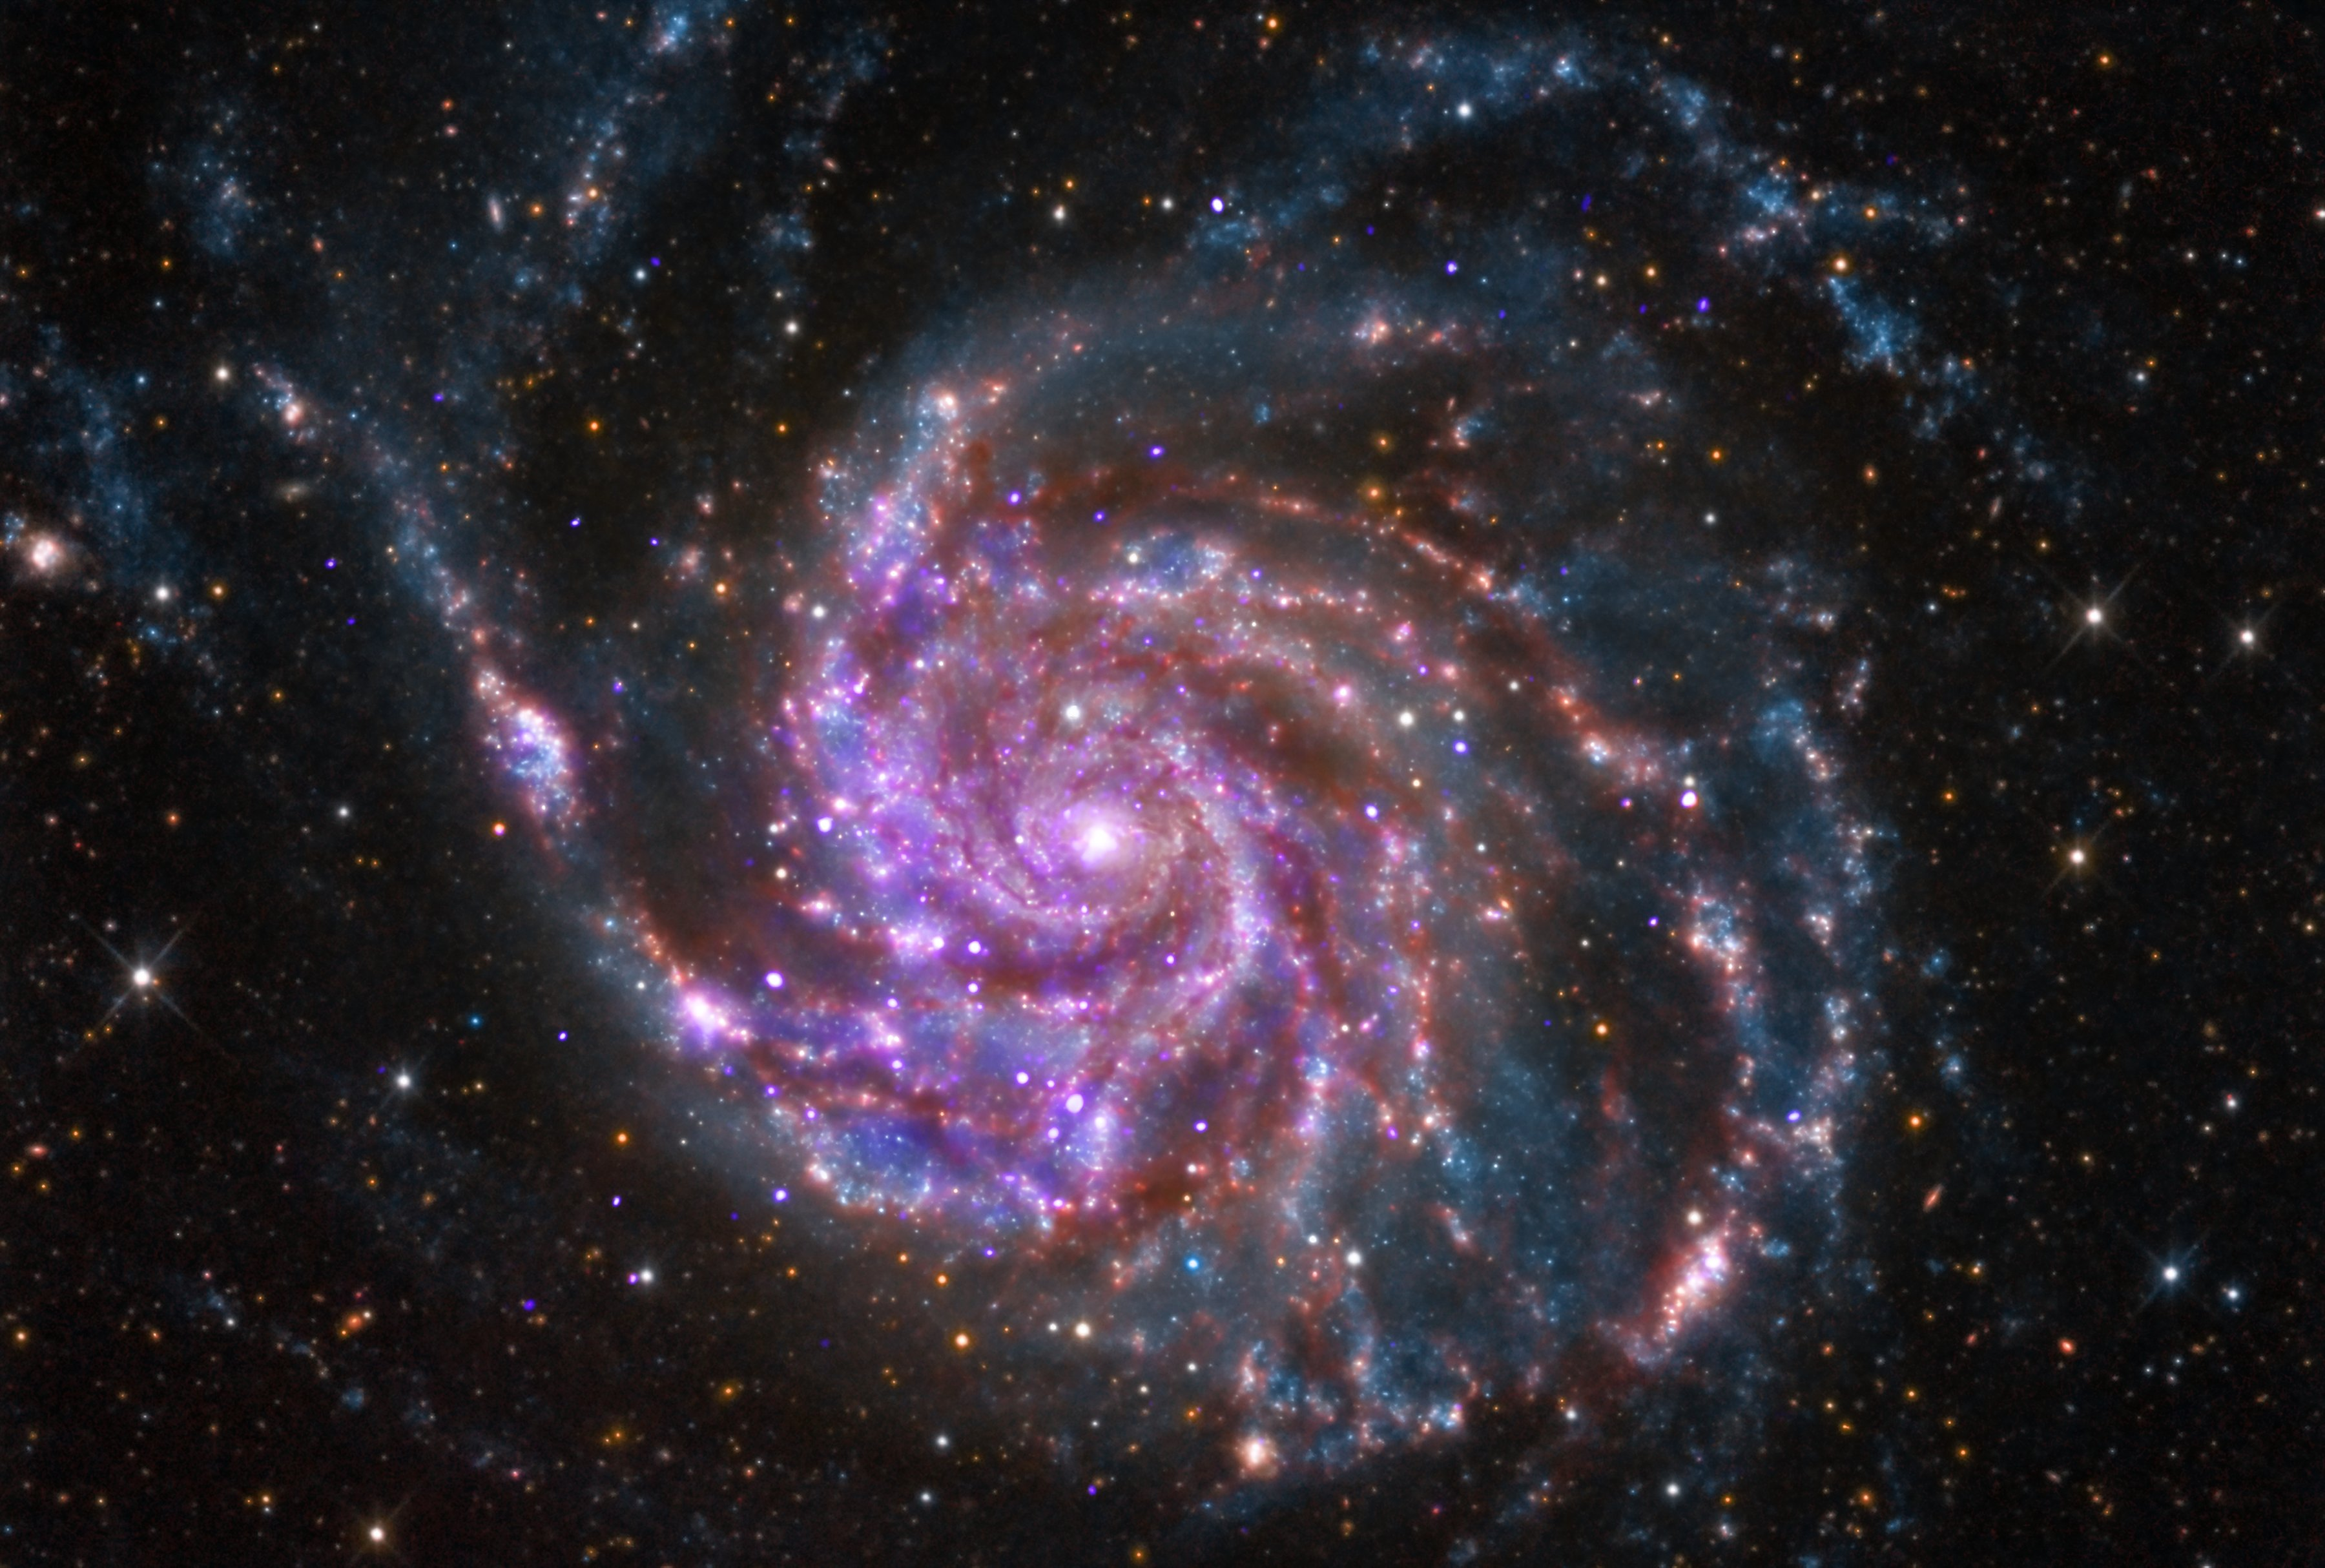
\includegraphics[width=3.5cm]{c1.introduction/system.01.jpg}}\qquad
    \only<3->{\includegraphics[width=2.5cm]{c1.introduction/system.02.png}}\\
    \only<4->{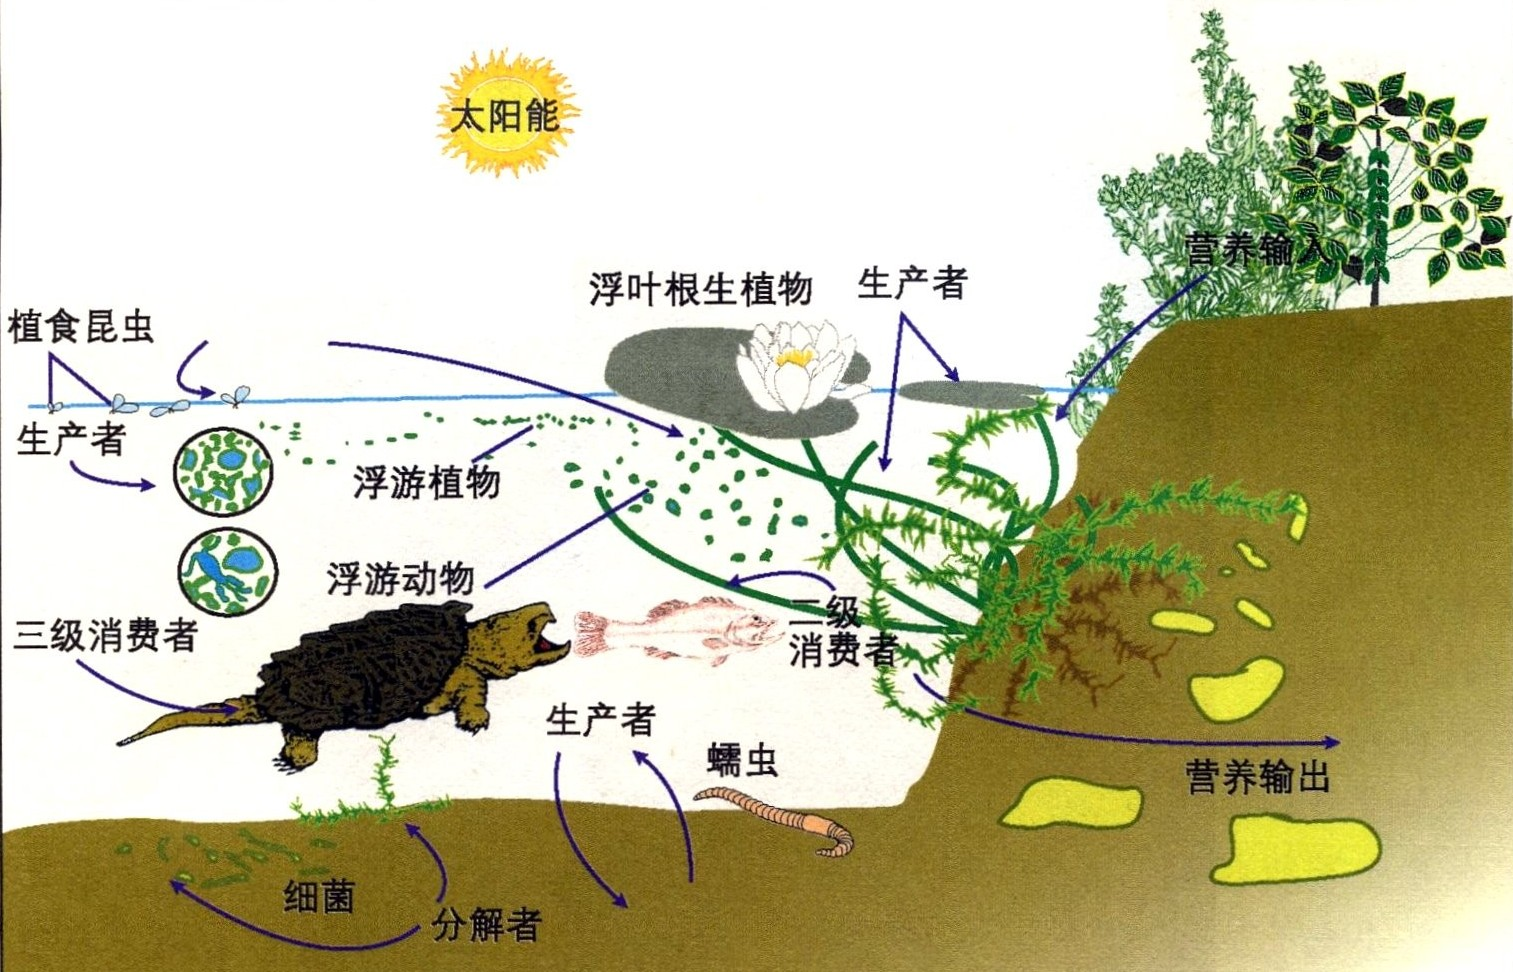
\includegraphics[width=3.5cm]{c1.introduction/system.03.jpg}}\quad
    \only<5->{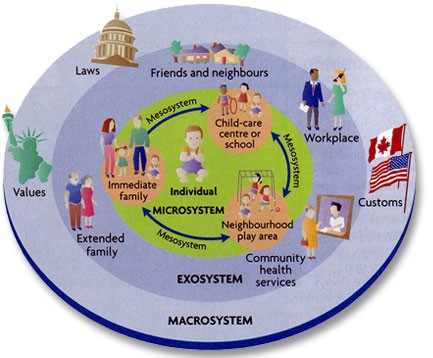
\includegraphics[width=3.2cm]{c1.introduction/system.04.jpg}}\quad
    \only<6->{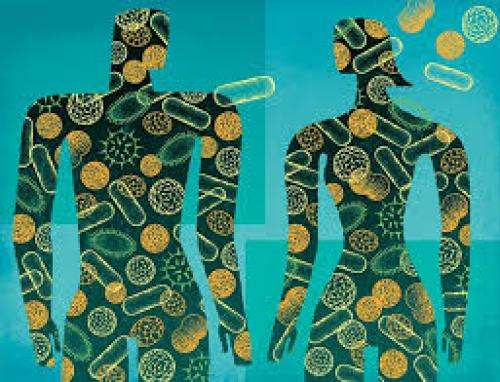
\includegraphics[width=3.2cm]{c1.introduction/system.05.jpg}}
  \end{figure}
\end{frame}

\begin{frame}
  \frametitle{概论 | 咬文嚼字 | 生命}
  \begin{block}{生命}
生命泛指一类具有稳定的物质和能量代谢现象并且能回应刺激、能进行自我复制(繁殖)的半开放物质系统。简单来说,也就是有生命机制的物体。生命个体一定会经历出生、成长、衰老和死亡。生命种群则在一代代个体的更替中经过自然选择发生进化以适应环境。\\
    \vspace{1em}
生命的最小单位是生物,生物是由一个或多个细胞组成,能够新陈代谢,维持恒定性,可以成长,回应刺激,可以繁殖甚至演化,以适应外界环境,继续繁殖并产生后代。在地球的生物圈内可以找到许多不同的生物,在这些生物中(包括植物、动物、真菌、原生生物、古菌及细菌),都有共同的特征,都是由以碳和水为基础的细胞构成,有其组织以及可以遗传的基因信息。\\
    \vspace{1em}
生物学是以研究生命为中心的科学。 
  \end{block}
\end{frame}

\begin{frame}[t]
  \frametitle{概论 | 咬文嚼字 | 生物}
  \begin{block}{生物}
    生物(organism,又称有机体)是指称类生命的个体,其最重要和基本的特征在于生物进行新陈代谢及遗传。\\
生物以细胞作为生命的基本单位,基因作为遗传的基本单元,进化是推动新物种的合成和创建的引擎。所有生物体的生存以消耗和转换能量,调节体内环境以维持稳定和重要的生命条件。
  \end{block}
  \begin{figure}
    \centering
    \only<2->{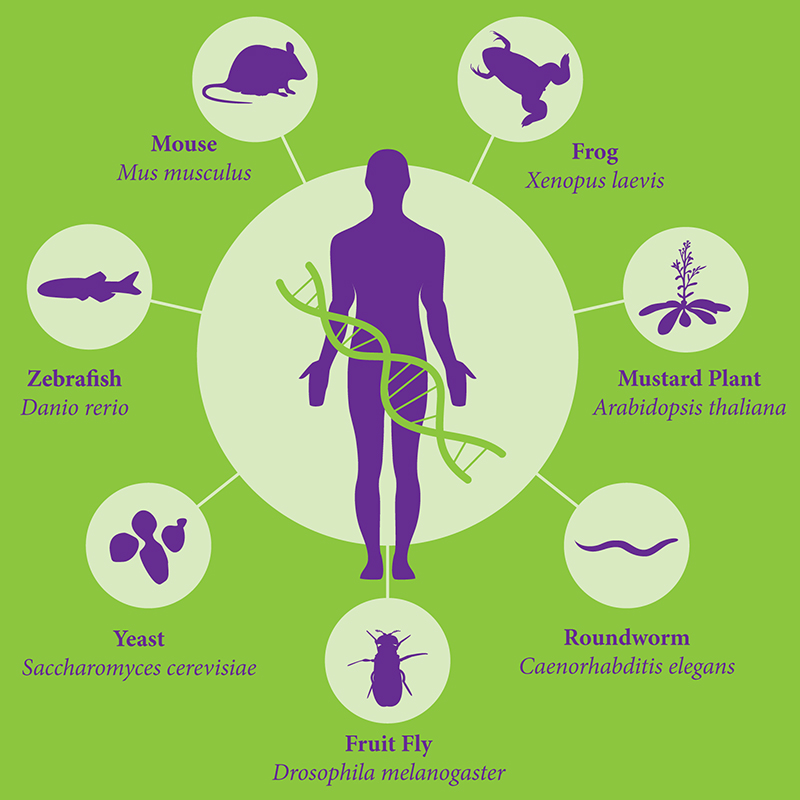
\includegraphics[width=4.5cm]{c1.introduction/organism.01.jpg}}\qquad
    \only<2->{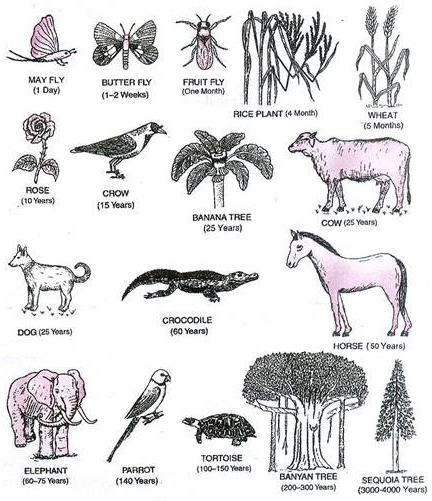
\includegraphics[width=4cm]{c1.introduction/organism.02.png}}
  \end{figure}
\end{frame}

\begin{frame}
  \frametitle{概论 | 咬文嚼字 | 科学}
  \begin{block}{科学}
    科学(science)是通过经验实证的方法,对现象(原来指自然现象,现泛指包括社会现象等现象)进行归因的学科。\\
    \vspace{1em}
人们习惯根据研究对象的不同把科学划分为不同的类别,传统的自然科学主要有生物学、物理学、化学、地质学和天文学。逻辑学和数学的地位比较特殊,它们是其它一切科学的论证基础和工具。
  \end{block}
  \begin{figure}
    \centering
    
\includegraphics[width=10cm]{c1.introduction/science.01.png}
  \end{figure}
\end{frame}

\begin{frame}
  \frametitle{概论 | 咬文嚼字 | 科学 vs. 真理/正确}
  \begin{block}{科学}
科学活动所得的知识是条件明确的(不能模棱两可或随意解读)、能经得起检验的,而且不能与任何适用范围内的已知事实产生矛盾。科学原仅指对自然现象之规律的探索与总结,但人文学科也被越来越多地冠以“科学”之名。\\
    \vspace{1em}
科学在认识自然的不同层面上设法解决各种具体的问题,强调预测结果的具体性和\textcolor{red}{可证伪性},这有别于空泛的哲学。\textcolor{red}{科学也不等同于寻求绝对无误的真理},而是在现有基础上,摸索式地不断接近真理。故科学的发展史就是一部人类对自然界的认识偏差的纠正史。因此\textcolor{red}{“科学”本身要求对理论要保持一定的怀疑性},因此它\textcolor{red}{绝不是“正确”的同义词}。
  \end{block}
\end{frame}

\begin{frame}
  \frametitle{概论 | 咬文嚼字 | 科学 | 发展的眼光}
  \begin{block}{中华人民共和国主席令}
根据中华人民共和国第十二届全国人民代表大会常务委员会第二十一次会议于2016年7月2日的决定:免去袁贵仁的教育部部长职务;任命陈宝生为教育部部长。
  \end{block}
  \begin{block}{中共中央政治局会议决定}
根据《中国共产党章程》、《中国共产党纪律处分条例》的有关规定,给予薄熙来开除党籍处分,待党的十七届七中全会予以追认;根据《中华人民共和国公务员法》的有关规定,给予薄熙来开除公职处分;将薄熙来涉嫌犯罪问题及犯罪问题线索移送司法机关依法处理。\\
\vspace{0.5em}
根据《中国共产党章程》、《中国共产党纪律处分条例》有关规定,决定给予徐才厚开除党籍处分,对其涉嫌受贿犯罪问题及问题线索移送最高人民检察院授权军事检察机关依法处理。
  \end{block}
\end{frame}

\begin{frame}
  \frametitle{概论 | 咬文嚼字 | 科学 | 发展的眼光}
  \begin{block}{圣旨}
奉天承运,皇帝诏曰:今有太监郭槐谋逆不端,奸心叵测。先皇乏嗣,不思永祚之忠诚;太后怀胎,遽遭兴妖之暗算。怀抱龙袱,不遵凤诏,寇宫人之志可达天;离却北阙,竟赴南清,陈总管之忠堪贯日。因泪痕,生疑忌,将明朗朗初吐宝珠,立毙杖下。假诅咒,进谗言,把气昂昂一点余忠,替死梁间。致令堂堂国母,廿载沉冤;受尽了背井离乡之苦。若非耿耿包卿一腔忠赤,焉得有还珠返壁之期。似此灭伦悖理,理当严审细推。按诏究问,依法重办。事关国典,理重君亲。钦交开封府严加审讯,上命钦哉!望诏谢恩。
  \end{block}
\end{frame}

\subsection{组分合成}
\begin{frame}
  \frametitle{概论 | 咬文嚼字 | 系统科学}
  \begin{block}{系统科学}
系统指的是由相互联系、相互作用的要素(或部分)组成的具有一定结构和功能的有机整体;准确来说,要素+结构=系统。\\
\vspace{1em}
从系统的角度观察研究客观世界的学科,就是系统科学。它研究的领域横跨自然科学,社会科学,却除去其中较为狭窄的物理、生物、心理、经济意义,而把研究重心放在探究各个系统的本质规律上。系统科学主要研究系统的要素(或元素),结构,和系统的行为(性质)。 
  \end{block}
\end{frame}

\begin{frame}
  \frametitle{概论 | 咬文嚼字 | 生命科学}
  \begin{block}{生命科学}
生命科学包括所有对生物(微生物、动物、植物等)进行研究的科学领域,也包括对相关领域的考量,比如生物伦理学。尽管目前生物学仍然是生命科学的中心,分子生物学和生物技术上的进展,使得生命科学正成为一个专精化、多学科交叉的领域。\\
    \vspace{1em}
生命科学的某些子学科对特定类型的生物进行研究。比如动物学研究动物,植物学研究植物。也有一些生命科学的子学科研究生物体在某些方面的共性,比如解剖学和遗传学。另外,像生物工程这样的学科则更专注于利用生物体研究出尖端技术。而生命科学的另一分支,神经科学则想要探明意识的本质。生命科学的不同研究领域之间有很大的重叠。\\
  \end{block}
\end{frame}

\begin{frame}
  \frametitle{概论 | 咬文嚼字 | 生物学}
  \begin{block}{生物学}
   生物学(biology)或称生物科学(biological sciences)、生命科学(life sciences),是自然科学的一大门类,由经验主义出发,广泛研究生命的所有方面,包括生命起源、演化、分布、构造、发育、功能、行为、与环境的互动关系,以及生物分类学等。\\
  \end{block}
  \begin{figure}
    \centering
    
\includegraphics[width=0.9\textwidth]{c1.introduction/biology.01.jpg}
  \end{figure}
\end{frame}

\begin{frame}
  \frametitle{概论 | 咬文嚼字 | 生物学 | 分支学科}
  \begin{block}{生物学分支学科}
现代生物学是一个庞大而兼收并蓄的领域,由许多分支和分支学科组成。生物学分支学科被研究生物体的规模和研究它们使用的方法所定义:生物化学考察生命的基本化学;分子生物学研究生物分子之间错综复杂的关系;植物学研究植物的生物学;细胞生物学检查所有生命的基本组成单位,细胞;生理学检查组织,器官,和生物体的器官系统的物理和化学的功能;进化生物学考察生命的多样性的产生过程;生态学考察生物在其环境如何相互作用。
  \end{block}
  \begin{figure}
    \centering
    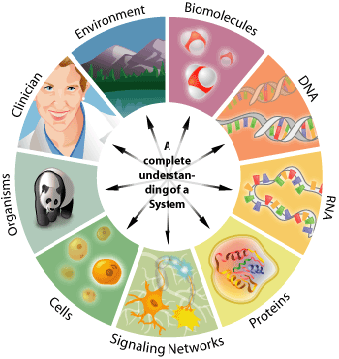
\includegraphics[width=0.28\textwidth]{c1.introduction/biology.subject.01.png}\qquad
    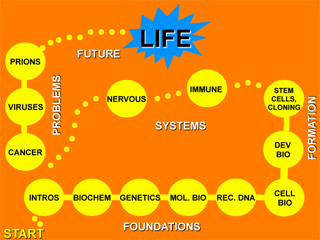
\includegraphics[width=0.38\textwidth]{c1.introduction/biology.subject.02.jpg}
  \end{figure}
\end{frame}

\begin{frame}
  \frametitle{概论 | 咬文嚼字 | 生物学 | 层次}
  \begin{figure}
    \centering
    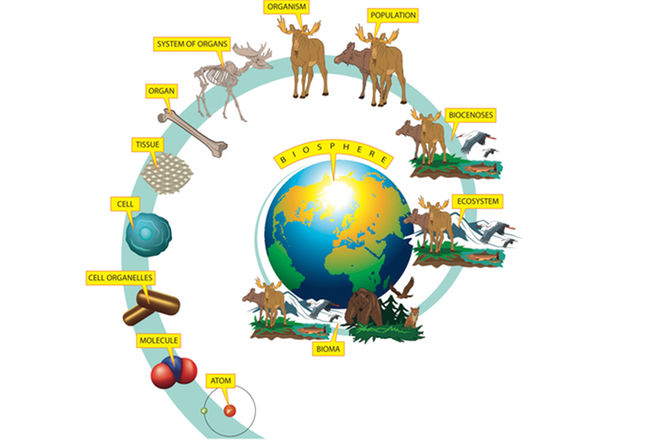
\includegraphics[width=0.9\textwidth]{c1.introduction/biological.hierarchy.01.jpg}
  \end{figure}
\end{frame}

\subsection{从组分到整体}
\begin{frame}
  \frametitle{概论 | 咬文嚼字 | 系统生物学}
  \begin{huge}
  \begin{center}
    \pause
    系统 \quad + \quad 科学 \quad = \quad 系统科学\\  
    \vspace{1em}
    \pause
    生物 \quad + \quad 科学 \quad = \quad 生物\textcolor{gray}{科}学\\ 
    \vspace{1em}
    \pause
    系统科学 \ + \ 生物\textcolor{gray}{科}学 \ = \ 系统生物学
  \end{center}
  \end{huge}
\end{frame}

\section{方法论}
\subsection{还原论}
\begin{frame}
  \frametitle{概论 | 方法论 | 还原论}
  \begin{block}{还原论}
还原论或还原主义(reductionism),是一种哲学思想,认为复杂的系统、事务、现象可以通过将其化解为各部分之组合的方法,加以理解和描述。\\
\vspace{1em}
还原论的思想在自然科学中有很大影响,例如认为化学是以物理学为基础,生物学是以化学为基础,等等。在社会科学中,围绕还原论的观点有很大争议,例如心理学是否能够归结于生物学,社会学是否能归结于心理学,政治学能否归结于社会学,等等。
  \end{block}
\end{frame}

\begin{frame}
  \frametitle{概论 | 方法论 | 还原论}
  \begin{figure}
    \centering
    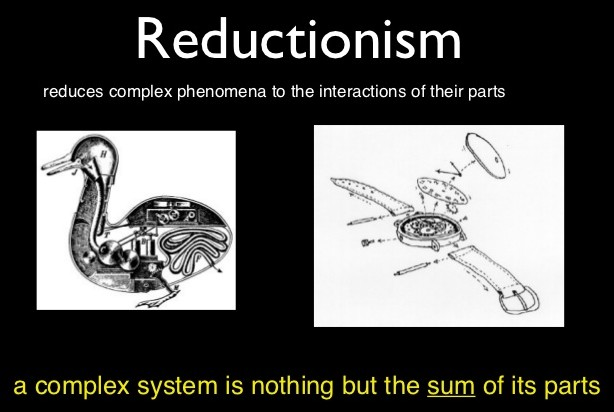
\includegraphics[width=0.9\textwidth]{c1.introduction/reductionism.01.jpg}
  \end{figure}
\end{frame}

\begin{frame}
  \frametitle{概论 | 方法论 | 科学统一论}
  \begin{block}{科学统一论}
科学统一论是某些科学哲学家对科学的一种看法,科学统一论主要认为所有的科学学科都形成一个统一的整体。\\
\vspace{1em}
举例说,一般人认为物理学和社会学等都是明显不同的学科,科学统一论者却认为,各种学科的差异只不过是对同一件事不同层面的了解,所以原则上,社会学是可以用物理学的观点去了解的。\\
\vspace{1em}
一般科学统一论者认为物理学是以最基础的概念去了解事物,化学的概念在理解层次上高于物理学,但一切化学概念都可以用物理学来解释,细胞生物学概念则高于化学,但是所有细胞运作都可以用化学概念去了解,个体生物学概念则高于细胞生物学,但一切对于生物整体的了解都可以用细胞生物学来解释等。
  \end{block}
\end{frame}

\begin{frame}
  \frametitle{概论 | 方法论 | 机械论}
  \begin{block}{机械论}
机械论(mechanism)是一种对于自然界的信念,认为自然界整体就是一个复杂的机器或工艺品,其不同组成部分间并没有内在联系。在此观点看来,物体或生物的行为可以从其组成部分和外界影响上来解释。\\
\vspace{1em}
哲学中的机械论观点有两种不同的指向。它们都是形而上学的观点,但有着不同的运用领域:第一个用于讨论自然界,第二个用于讨论人和人的心灵。为明确起见,我们或许可以将此两者分别称为宇宙机械论(universal mechanism)和人类机械论(anthropic mechanism)。
  \end{block}
\end{frame}

\begin{frame}
  \frametitle{概论 | 方法论 | 机械论}
  \begin{figure}
    \centering
    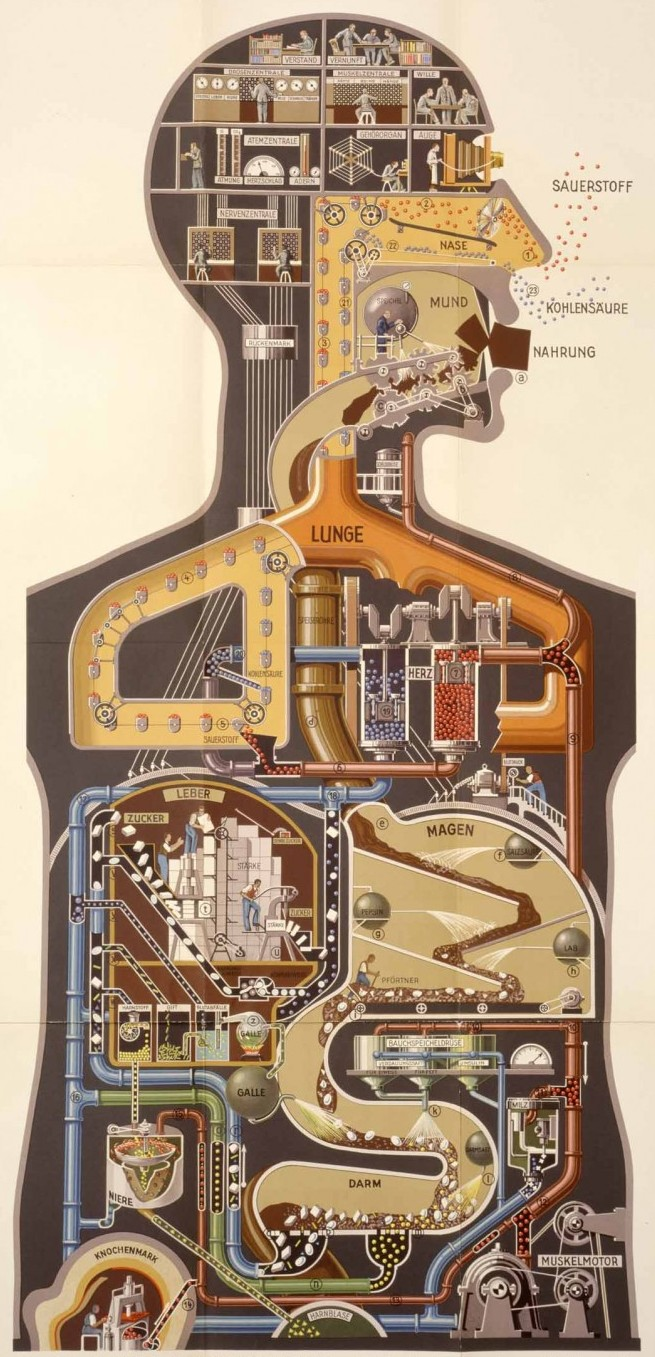
\includegraphics[width=0.55\textwidth]{c1.introduction/mechanism.01.jpg}
  \end{figure}
\end{frame}

\begin{frame}
  \frametitle{概论 | 方法论 | 基因决定论}
  \begin{block}{基因决定论}
所谓“基因决定论”是指这样一种思想倾向与理论方法:将基因信息与人的行为、心理活动一一简单对应,并以前者解释后者,认为一个人的基因信息内容决定了他/她自身的行为方式与心理内容。\\
\vspace{1em}
  生命的各种性质和活动都是受基因控制的,甚至人类的精神活动也在基因的控制之下。
  \end{block}
\end{frame}

\begin{frame}
  \frametitle{概论 | 方法论 | 基因决定论}
  \begin{figure}
    \centering
    \only<2->{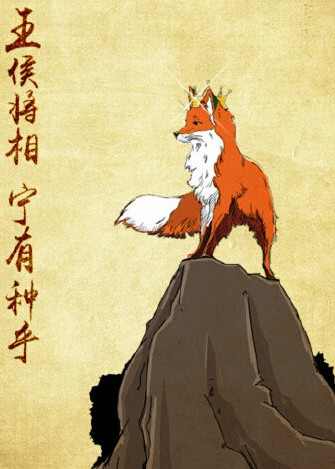
\includegraphics[width=0.4\textwidth]{c1.introduction/gene.determinism.01.jpg}}\qquad
    \only<3->{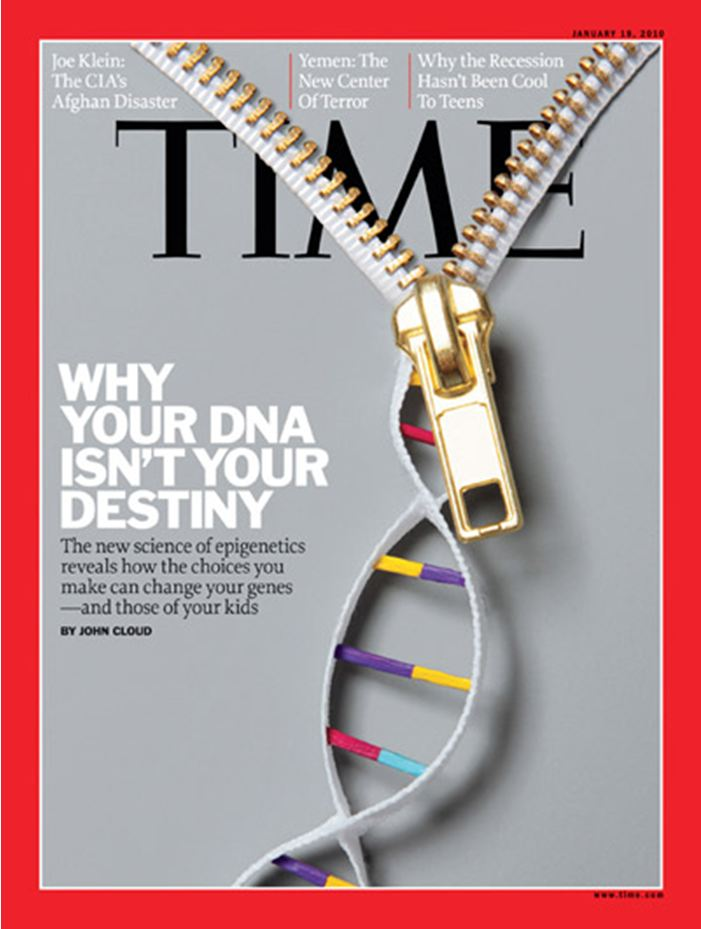
\includegraphics[width=0.42\textwidth]{c1.introduction/epigenetics.01.jpg}}
  \end{figure}
\end{frame}

\subsection{整体论}
\begin{frame}
  \frametitle{概论 | 方法论 | 系统论}
  \begin{block}{系统论}
系统论运用完整性、集中性、等级结构、终极性、逻辑同构等概念,研究适用于一切综合系统或子系统的模式、原则和规律,并力图对其结构和功能进行数学描述。系统强调整体与局部、局部与局部、整体与外部环境之间的有机联系,具有整体性、动态性和目的性三大基本特征。作为一种指导思想,系统论要求把事物当作一个整体或系统来考察。\\
\vspace{0.5em}
系统论的核心思想是系统的整体观念。任何系统都是一个有机的整体,它不是各个部分的机械组合或简单相加,系统的整体功能是各要素在孤立状态下所没有的性质。\\
\vspace{0.5em}
系统论的基本思想方法,就是把所研究和处理的对象,当作一个系统,分析系统的结构和功能,研究系统、要素、环境三者的相互关系和变动的规律性,并优化系统观点看问题,世界上任何事物都可以看成是一个系统,系统是普遍存在的。大至渺茫的宇宙,小至微观的原子,一粒种子、一群蜜蜂、一台机器、一个工厂、一个学会团体……都是系统,整个世界就是系统的集合。
  \end{block}
\end{frame}

\begin{frame}
  \frametitle{概论 | 方法论 | 整体论}
  \begin{block}{整体论}
整全观(holism)的主张,是一个系统(宇宙、人体等)中各部分为一有机之整体,而不能割裂或分开来理解。根据此一观点,分析整体时若将其视作部分的总和,或将整体化约为分离的元素,将难免疏漏。\\
\vspace{1em}
许多原始文明也有整全观的概念,例如北美或澳洲的原住民相信他们跟土地、神灵、动植物的联系,并体现在宗教仪式之中。中国古代儒道思想有“天人合一”,中医学说明了整全观如何应用在实用性的学科——它将人体各部分视为一有机整体,而不单是器官的整合。要医治病人须保持整个人阴阳调和,而非单一器官的问题。中医也是现代整全医疗中的代表之一。
  \end{block}
\end{frame}

\begin{frame}
  \frametitle{概论 | 方法论 | 整体论}
  \begin{figure}
    \centering
    
\includegraphics[width=0.42\textwidth]{c1.introduction/holism.01.jpg}\quad
    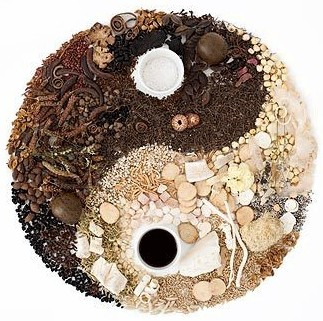
\includegraphics[width=0.5\textwidth]{c1.introduction/holism.03.jpg}
  \end{figure}
\end{frame}

\subsection{还原论 vs. 整体论}
\begin{frame}
  \frametitle{概论 | 方法论 | 还原论 vs. 整体论}
还原论常常被视为对立于整全观。科学上的还原论的主张为:在一个复杂系统里,组成部分的行为可以解释整体系统的表现。18至20世纪流行于科学家之间的哲学逻辑实证论,其中一个信念就是科学研究是阶层式的:物理→化学→生物学→心理学→社会科学,化学的法则可以用物理学解释,生物学的法则可以用化学去解释。\\
\vspace{1em}
在学术研究上,对复杂系统的研究,令偏向抽象事物的研究者明白“还原”不足以解释一个复杂系统内部交叉产生的现象;在现实问题里,例如处理疾病、贫穷、经济、城市规划、惯性收视等问题时,经常需要跨学科的合作;在社会上,20世纪中人们开始重视生态圈、环境保护,国家政府过于追求国内生产总值(GDP)以致忽略国民的生活素质,有人提出国民幸福总值以取代GDP。这些事件,都可以说体现人们更重视整全观。
\end{frame}

\begin{frame}
  \frametitle{概论 | 方法论 | 还原论 vs. 整体论}
  \begin{figure}
    \centering
    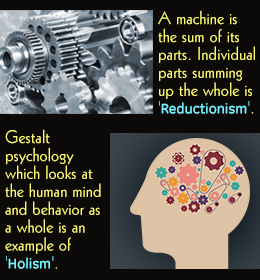
\includegraphics[width=0.6\textwidth]{c1.introduction/reductionism.vs.holism.01.jpg}
  \end{figure}
\end{frame}

\begin{frame}
  \frametitle{概论 | 方法论 | 补遗}
  \begin{figure}
    \centering
    \only<1->{
\includegraphics[width=0.4\textwidth]{c1.introduction/nonscience.01.jpg}}\qquad
    \only<2->{
\includegraphics[width=0.3\textwidth]{c1.introduction/liro.01.png}}\\
    \vspace{1em}
    \only<3->{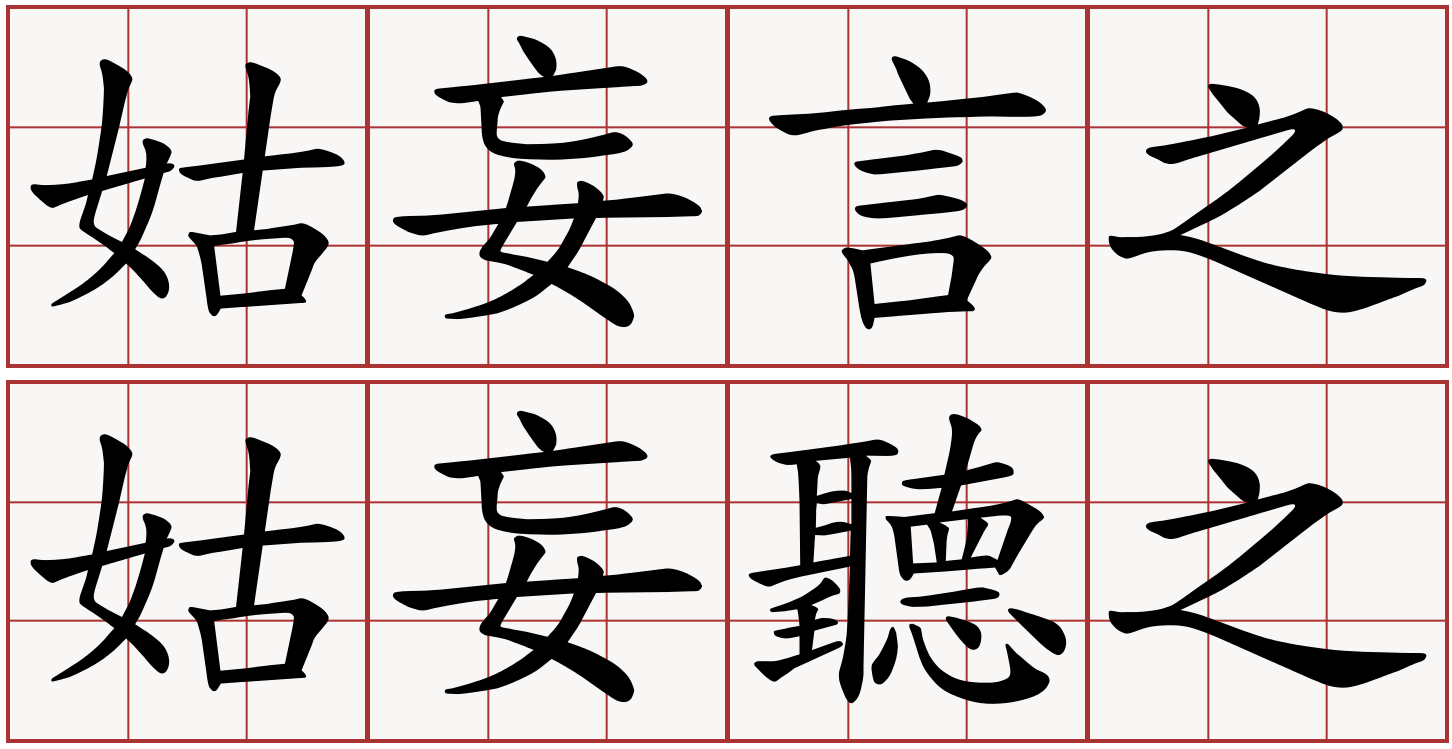
\includegraphics[width=0.4\textwidth]{c1.introduction/liro.10.png}}
  \end{figure}
\end{frame}

\section{系统生物学}
\subsection{发展历史}
\begin{frame}
  \frametitle{概论 | 系统生物学 | 历史}
  \begin{figure}
    \centering
    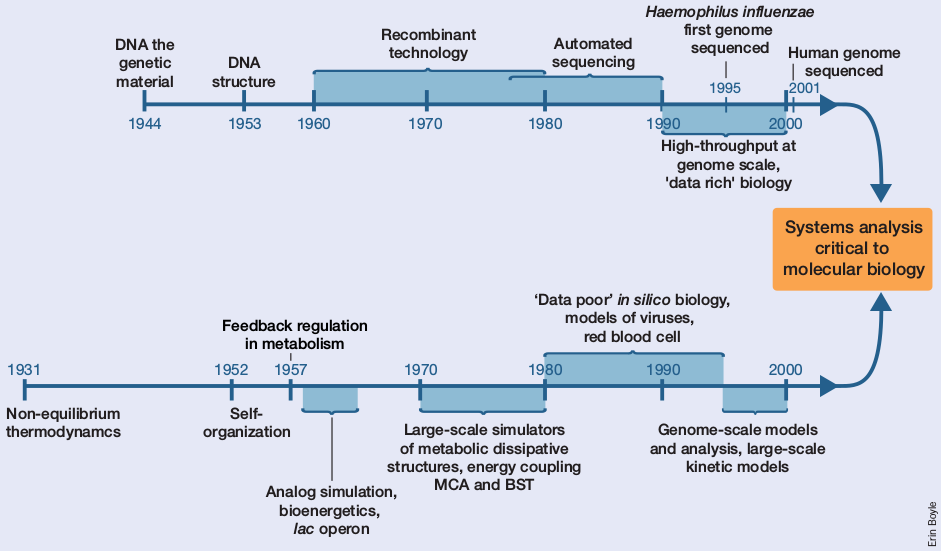
\includegraphics[width=0.9\textwidth]{c1.introduction/sb.history.01.png}
  \end{figure}
\end{frame}

\begin{frame}
  \frametitle{概论 | 系统生物学 | 历史 | 事件}
  \begin{itemize}
    \item 系统科学:最初源自对还原论、机械论反省的有机体思维、综合哲学
    \item 相关研究$\Rightarrow$将生命现象看作自组织化系统:C.贝尔纳与W.B.坎农对生物稳态现象的揭示,贝塔郎菲的一般系统论与理论生物学,维纳与艾什比的控制论,香农的信息论,I.普里戈津的耗散结构理论
    \item 1950年代,系统心理学
    \item 1950年,贝塔郎菲,《物理学与生物学中的开放系统理论》,创立一般系统论,奠基了系统生物学基础
  \end{itemize}
\end{frame}

\begin{frame}
  \frametitle{概论 | 系统生物学 | 历史 | 事件(续)}
  \begin{itemize}
    \item 1968年,国际系统论与生物学(systems theory and biology)会议,提出以系统论(整合的)方法研究生物学的体系
    \item 1970-80年代,系统论与生物学、系统生物学等概念发表,系统生态学、系统生理学等学科先后建立与成熟,细胞生物学、生物化学与分子生物学发展
    \item 1989年,美国,生物化学系统论与计算机模型研究的国际会议,研讨生物系统的计算机方法、数学模型与定量研究
    \item 21世纪伊始,系统生物学的发展进入了细胞信号传导与基因表达调控研究的细胞、分子系统生物学时期,国际、国内的系统与合成生物学、系统遗传学等研究机构纷纷建立,进入系统生命科学时代
    \item 2000年,第一届国际系统生物学会(1st International Conference on Systems Biology;ICSB 2000)
    \item 2000年,莱诺伊·胡德、阿兰·阿德雷姆及鲁迪·艾伯索尔德,系统生物学研究所(Institute for Systems Biology)
  \end{itemize}
\end{frame}

\begin{frame}
  \frametitle{概论 | 系统生物学 | 历史 | 分子生物学 vs. 系统生物学}
  \begin{figure}
    \centering
    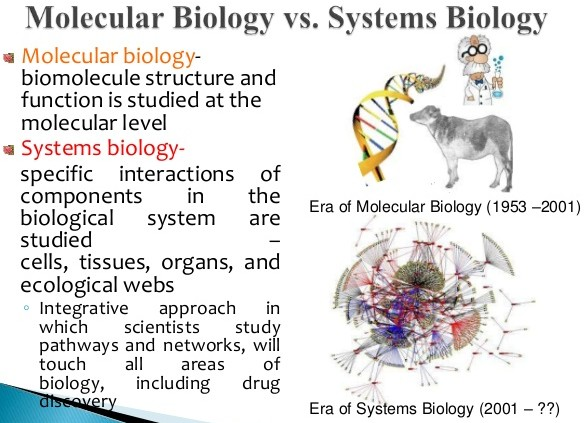
\includegraphics[width=0.9\textwidth]{c1.introduction/sb.history.02.jpg}
  \end{figure}
\end{frame}

\begin{frame}
  \frametitle{概论 | 系统生物学 | 历史 | 分子生物学 vs. 系统生物学}
  \begin{block}{Molecular $\Rightarrow$ System}
  Systems biology is a natural extension of molecular biology, and can be defined as ``biology after the identification of key genes".
  \end{block}
\end{frame}

\begin{frame}
  \frametitle{概论 | 系统生物学 | 历史 | 组学 $\rightarrow$ 系统生物学}
  \begin{figure}
    \centering
    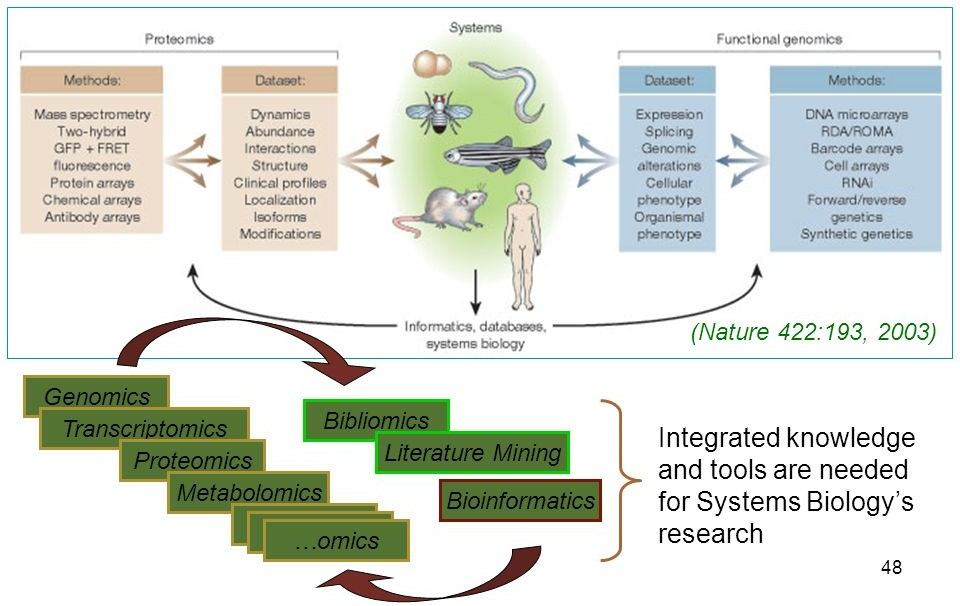
\includegraphics[width=0.9\textwidth]{c1.introduction/sb.history.05.jpg}
  \end{figure}
\end{frame}

\subsection{学科定义}
\begin{frame}
  \frametitle{概论 | 系统生物学 | 定义}
  \begin{block}{莱诺伊·胡德,2001}
    系统生物学是将DNA、RNA、蛋白质以及三者彼此之间的交互作用等信息加以整合,并运用这些资料去建立出数学计量模型,以期能掌握所有生物基因与组织间的关系及运作。\\
\vspace{1em}
系统生物学的研究过程是先取得一个生物、组织或细胞系统,辨识出各种内部因素,在获得DNA、RNA及蛋白质相互作用及信息网络方面整合所获得的信息,然后开发出能描述系统结构和行为的数学模型,最后可以借由此一个模型系统,使这个系统可以自动执行所需的功能。\\
\vspace{1em}
系统生物学是结合许多不同学科的领域,透过彼此相互的网状合作,针对一个生物现象所进行的研究。
  \end{block}
\end{frame}

\begin{frame}
  \frametitle{概论 | 系统生物学 | \textcolor{red}{定义}}
  \begin{block}{Hood,2004}
系统生物学是研究一个生物系统中所有组成成分(基因、mRNA、蛋白质等)的构成,以及在特定条件下这些组分间的相互关系,并通过计算生物学建立一个数学模型来定量描述和预测生物功能、表型和行为的学科。
  \end{block}
\end{frame}

\begin{frame}
  \frametitle{概论 | 系统生物学 | 定义}
  \begin{block}{北野宏明}
系统生物学的研究可以包含四大部分,分别利用信息科学、分析、技术、基因组学四者形成环型而连续的关系,建立出一个新的研究模式,并且利用这一模式所发展的一系列的工具来解决生物学家所面临的研究问题。
  \end{block}
\end{frame}

\begin{frame}
  \frametitle{概论 | 系统生物学 | 定义}
  \begin{block}{日本}
系统生物学是生物学的一个新领域,其目的在于在系统层次上理解生物系统,力求阐述作为一个系统的生物系统,并重点着眼于以下四个问题:
  \begin{enumerate}
    \item 系统结构的阐述;
    \item 系统行为的分析;
    \item 控制系统的方法;
    \item 如何设计系统。
  \end{enumerate}
  \end{block}
\end{frame}

\begin{frame}
  \frametitle{概论 | 系统生物学 | \textcolor{red}{定义}}
  \begin{block}{杨胜利,2004}
系统生物学是在细胞、组织、器官和生物体水平上研究结构和功能各异的生物分子及其相互作用,并通过计算生物学定量阐明和预测生物功能、表型和行为。\\
\vspace{1em}
系统生物学将在基因组测序基础上完成DNA序列到生命的过程,这是逐步整合、优化的过程,系统生物学的发展预计需要一个世纪或更长的时期,因此常把系统生物学称为21世纪的生物学。
  \end{block}
\end{frame}

\begin{frame}
  \frametitle{概论 | 系统生物学 | 定义}
  \begin{block}{维基百科}
系统生物学(systems biology),是一个试图整合不同层次信息以理解生物系统如何行使功能的学术领域。通过研究某生物系统各不同部分之间的相互关系和相互作用(例如,与细胞信号传送、代谢通路、细胞器、细胞、生理系统与生物等相关的基因和蛋白网络),系统生物学期望最终能够建立整个系统的可理解模型。系统生物学大量使用数学的和计算技术的模型。\\
\vspace{1em}
系统生物学开始于对基因和蛋白质的研究,该研究使用高通量技术来测定某物种在给定条件干涉下基因组和蛋白质组的变化。研究基因组的高通量技术包括用来测定mRNA变化的生物芯片技术。高通量蛋白质组学方法包括质谱,该技术用于鉴定蛋白质,检测蛋白修饰和量化蛋白质表达水平。
  \end{block}
\end{frame}

\begin{frame}
  \frametitle{概论 | 系统生物学 | 定义}
  \begin{block}{第二届国际系统生物学会,2001}
系统生物学是对生物体整个过程做一全面性的定量研究,并非以生物体的某一部分为对象。目的是要建立模式并以实验来证实其可预测的生物体的表现。\\
\vspace{1em}
简单的说,这样的研究方法就是利用信息科学及微机电工程的技术来研究生物学的问题,最后并希望能够利用电脑运算的结果,来预测细胞、器官、系统甚至完整生物体的表现。
  \end{block}
\end{frame}

\begin{frame}
  \frametitle{概论 | 系统生物学 | 定义}
  \begin{figure}
    \centering
    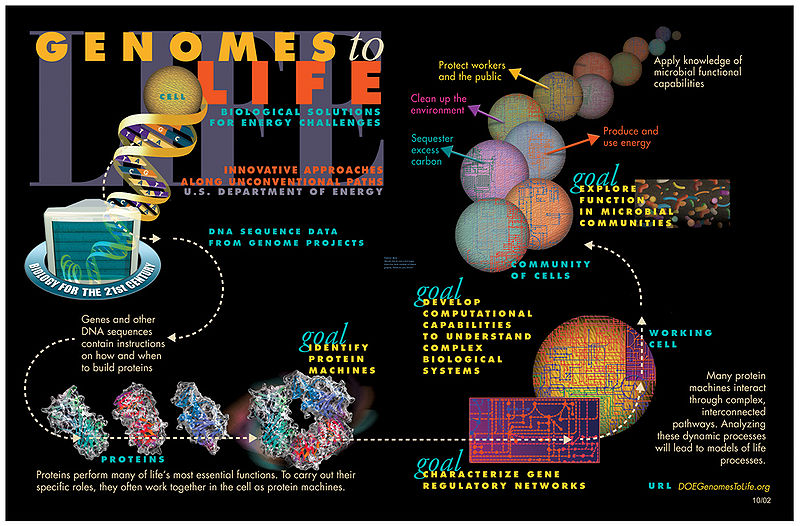
\includegraphics[width=0.9\textwidth]{c1.introduction/sb.02.jpg}
  \end{figure}
\end{frame}

\begin{frame}
  \frametitle{概论 | 系统生物学 | 定义}
  \begin{figure}
    \centering
    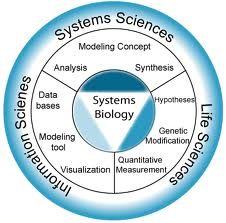
\includegraphics[width=0.6\textwidth]{c1.introduction/sb.01.jpg}
  \end{figure}
\end{frame}

\subsection{研究内容}
\begin{frame}
  \frametitle{概论 | 系统生物学 | \textcolor{red}{内容}}
  \begin{block}{湿实验}
采用高通量实验技术,通过众多组学,在整体和动态研究水平上积累数据并在挖掘数据时发现新规律、新知识,提出新概念。
  \end{block}
  \pause
  \begin{block}{干实验}
通过计算生物学建立生物模型,根据被研究的真实系统的模型,利用计算机进行实验研究。
  \end{block}
\end{frame}

\begin{frame}
  \frametitle{概论 | 系统生物学 | 内容}
  \begin{figure}
    \centering
    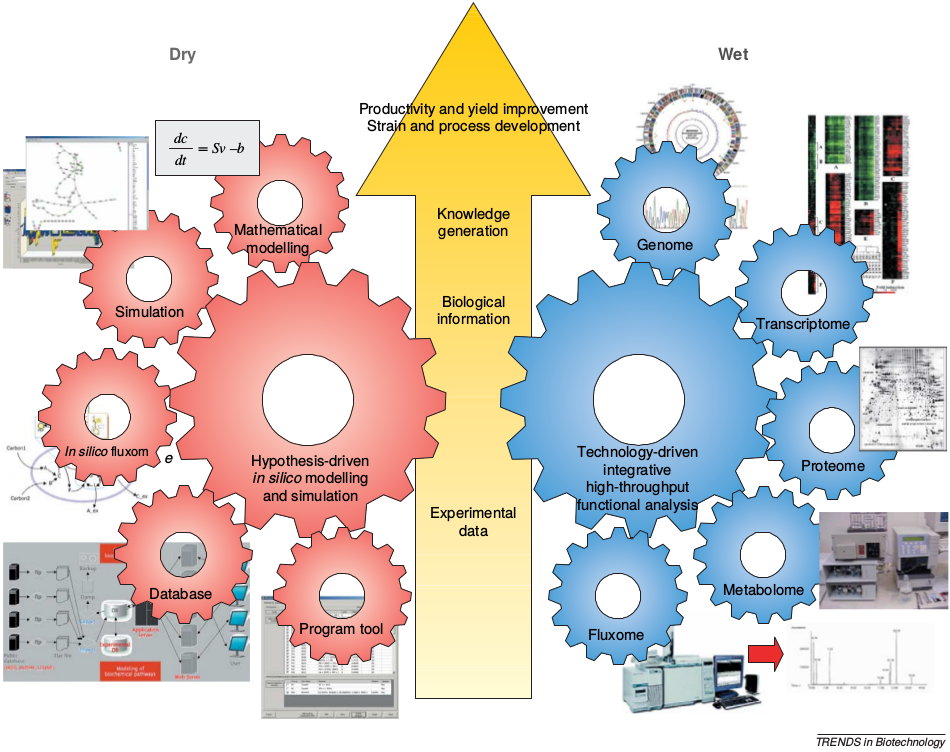
\includegraphics[width=0.8\textwidth]{c1.introduction/sb.content.03.png}
  \end{figure}
\end{frame}

\begin{frame}
  \frametitle{概论 | 系统生物学 | 内容}
  \begin{figure}
    \centering
    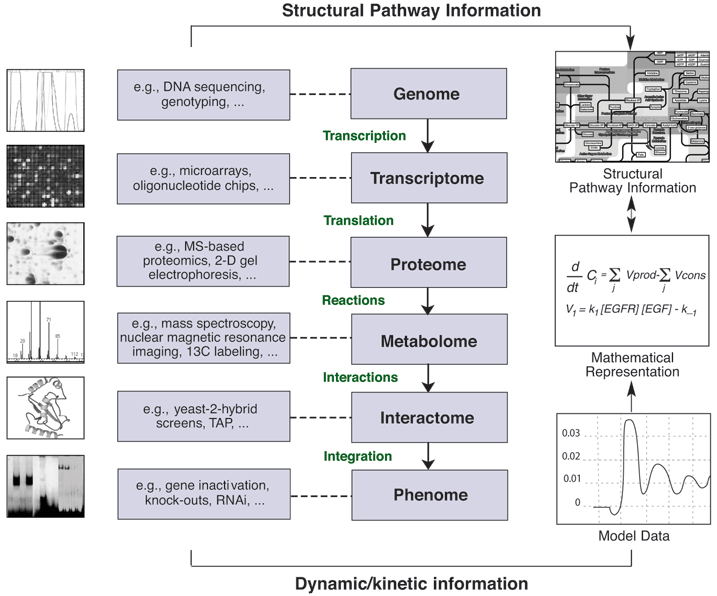
\includegraphics[width=0.8\textwidth]{c1.introduction/sb.content.01.png}
  \end{figure}
\end{frame}

\subsection{工作流程}
\begin{frame}
  \frametitle{概论 | 系统生物学 | \textcolor{red}{流程}}
  \begin{columns}
    \column{0.35\textwidth}
    \begin{block}{流程}
  \begin{enumerate}
    \item 研究组分,构建模型
    \item 改变条件,观测变化
    \item 比较结果,修订模型
    \item 重新实验,继续修订
  \end{enumerate}
    \end{block}
    \column{0.65\textwidth}
  \begin{figure}
    \centering
    \only<2->{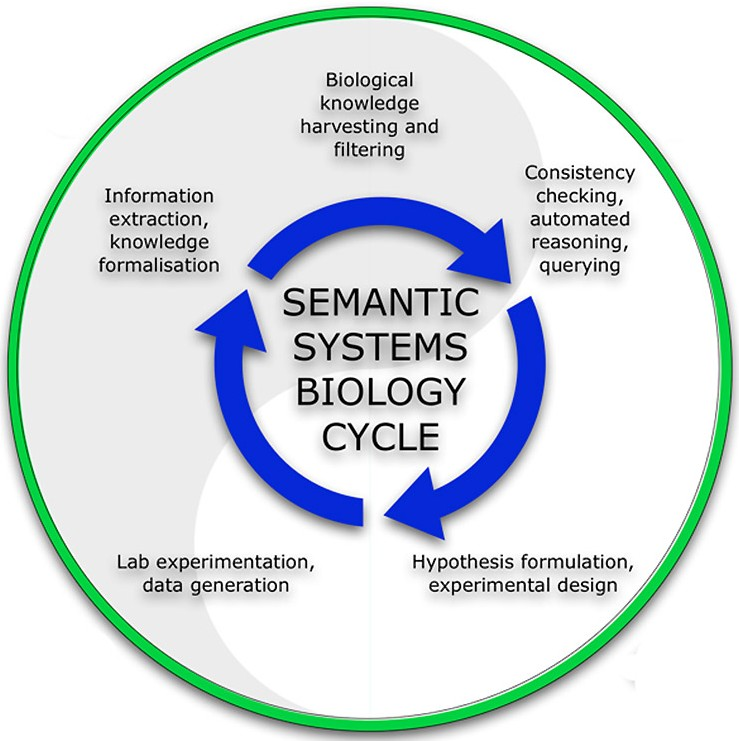
\includegraphics[width=0.8\textwidth]{c1.introduction/sb.workflow.01.jpg}}
  \end{figure}
  \end{columns}
\end{frame}

\begin{frame}
  \frametitle{概论 | 系统生物学 | 流程}
  \begin{figure}
    \centering
    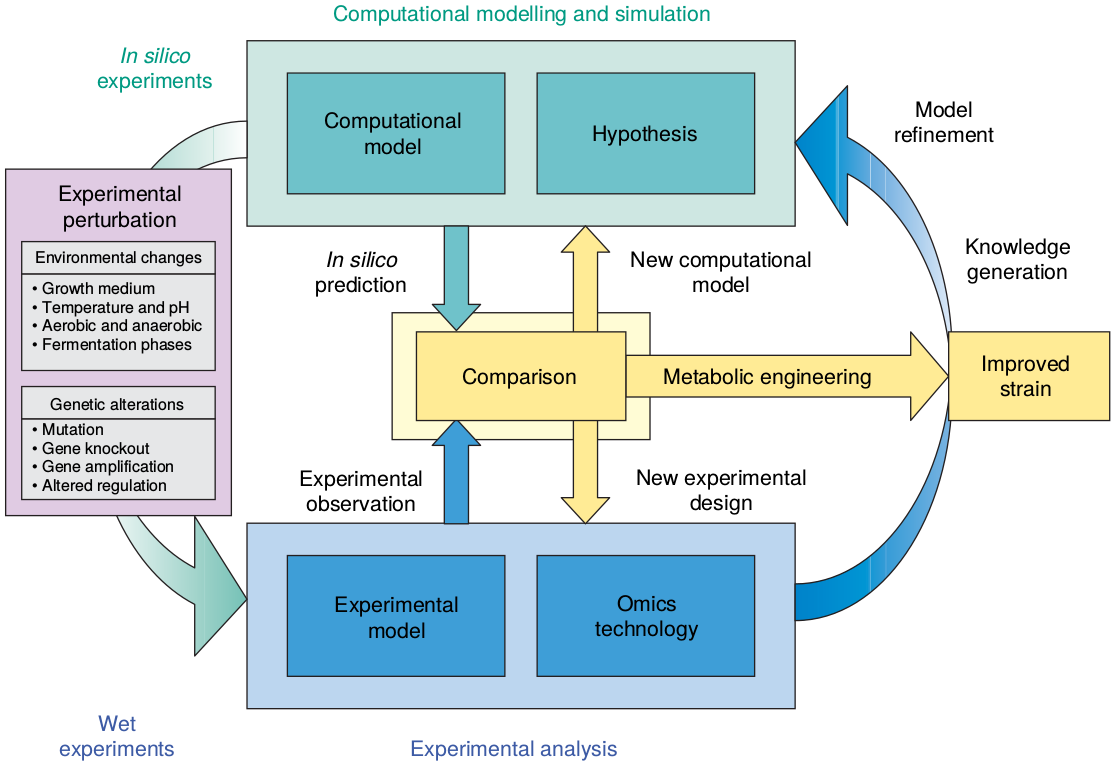
\includegraphics[width=0.9\textwidth]{c1.introduction/sb.workflow.02.png}
  \end{figure}
\end{frame}

\begin{frame}
  \frametitle{概论 | 系统生物学 | 流程}
  \begin{figure}
    \centering
    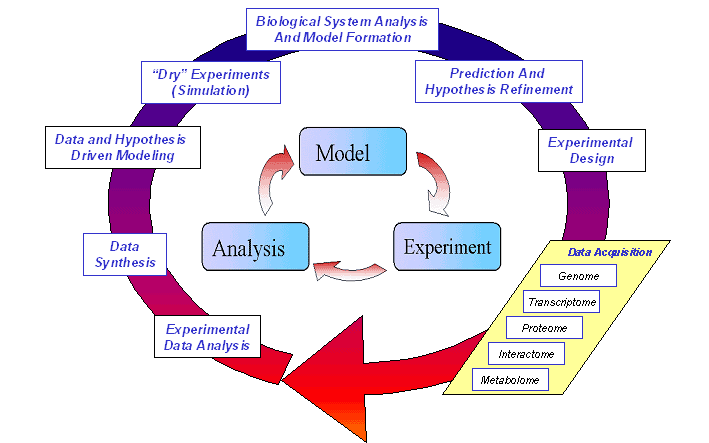
\includegraphics[width=0.9\textwidth]{c1.introduction/sb.workflow.03.png}
  \end{figure}
\end{frame}

\begin{frame}
  \frametitle{概论 | 系统生物学 | 流程}
  \begin{figure}
    \centering
    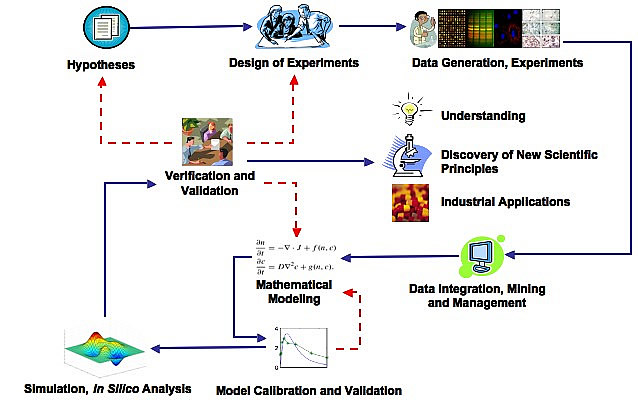
\includegraphics[width=0.9\textwidth]{c1.introduction/sb.workflow.04.jpg}
  \end{figure}
\end{frame}

\begin{frame}
  \frametitle{概论 | 系统生物学 | 流程}
  \begin{figure}
    \centering
    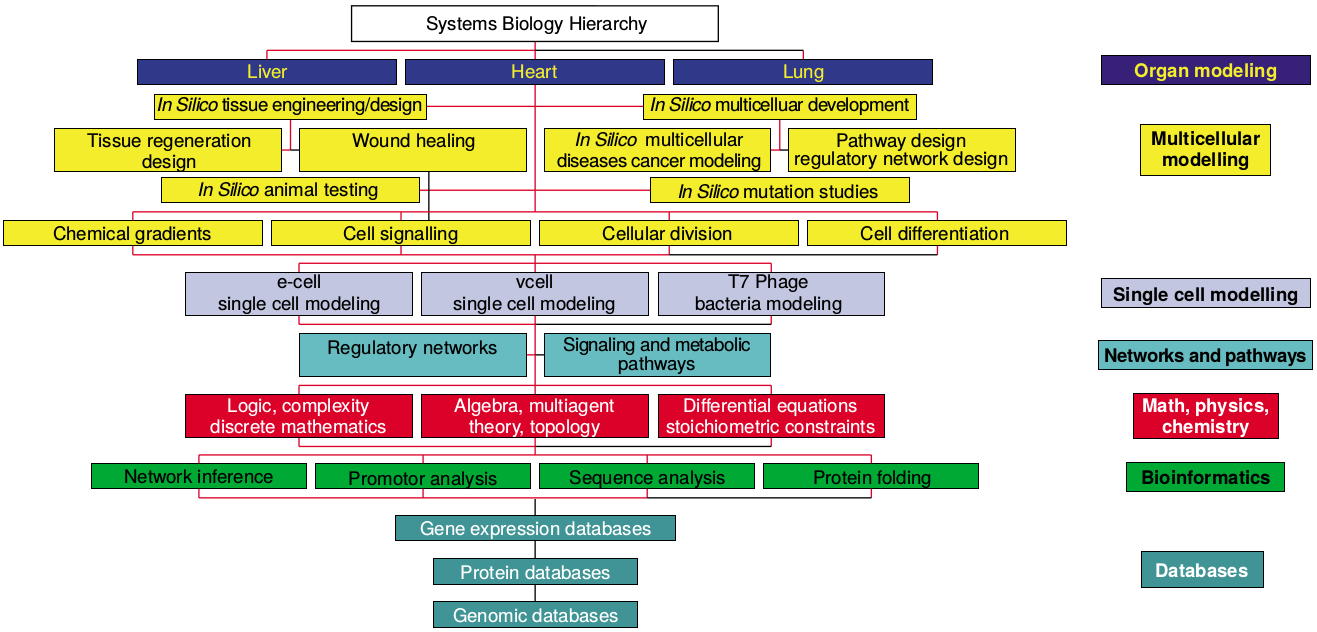
\includegraphics[width=\textwidth]{c1.introduction/sb.workflow.05.png}
  \end{figure}
\end{frame}

\begin{frame}
  \frametitle{概论 | 系统生物学 | 流程}
  \begin{figure}
    \centering
    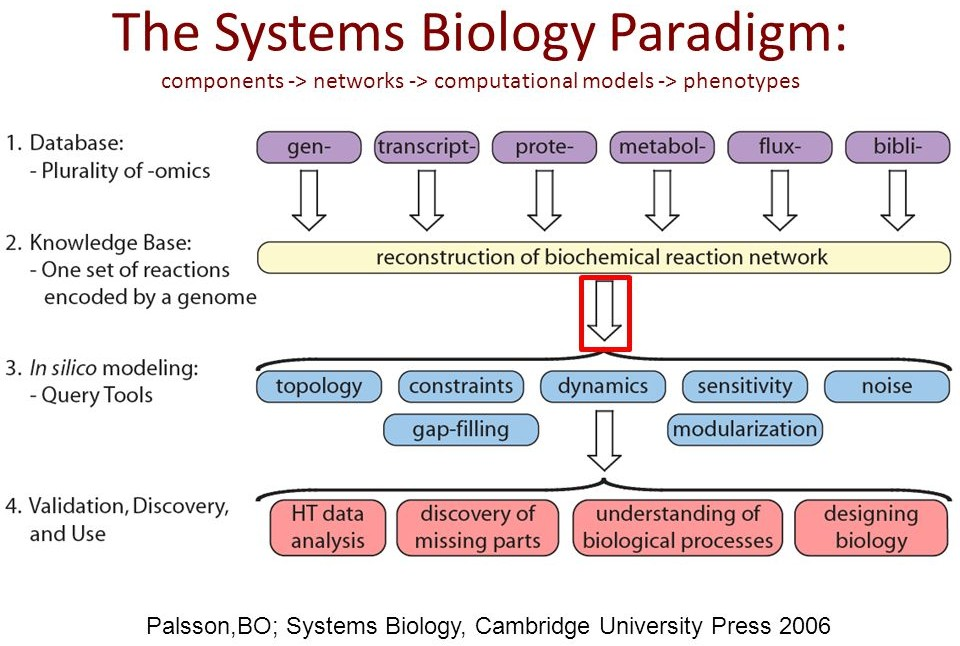
\includegraphics[width=0.9\textwidth]{c1.introduction/sb.workflow.06.jpg}
  \end{figure}
\end{frame}

\begin{frame}
  \frametitle{概论 | 系统生物学 | 流程}
  \begin{figure}
    \centering
    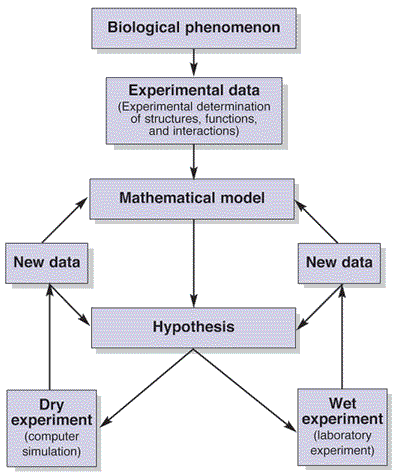
\includegraphics[width=0.5\textwidth]{c1.introduction/sb.workflow.07.png}
  \end{figure}
\end{frame}

\subsection{研究方法}
\begin{frame}
  \frametitle{概论 | 系统生物学 | 方法}
  \begin{figure}
    \centering
    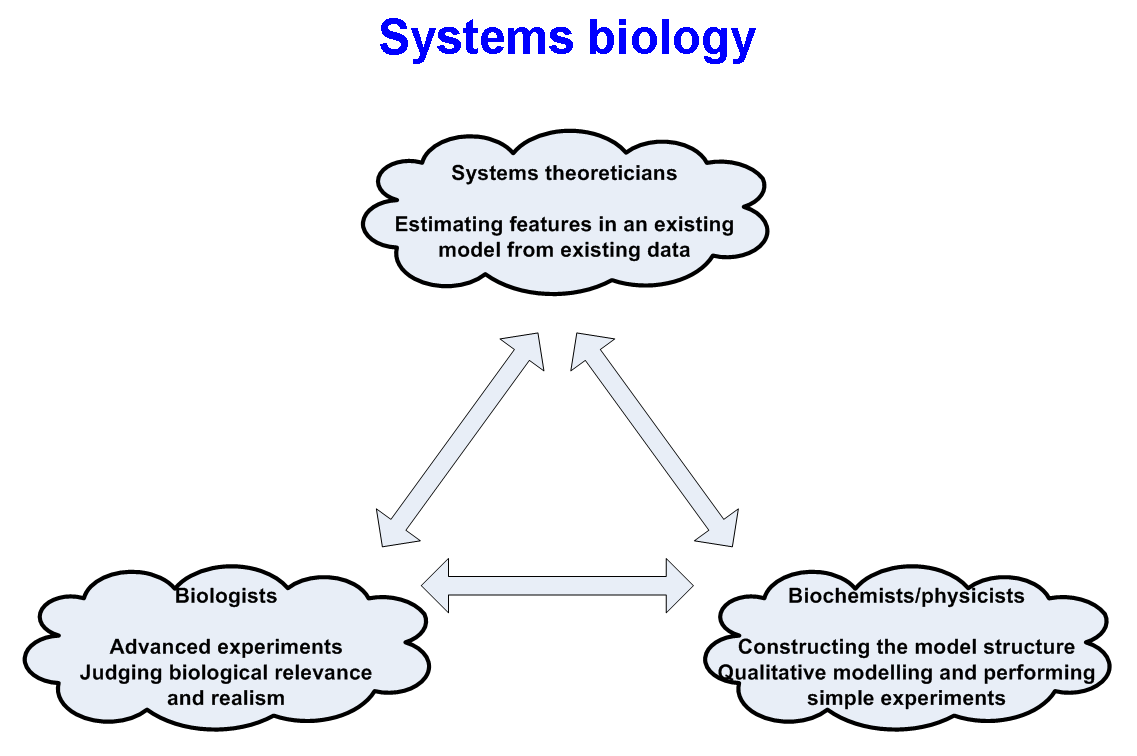
\includegraphics[width=0.9\textwidth]{c1.introduction/sb.method.01.png}
  \end{figure}
\end{frame}

\begin{frame}
  \frametitle{概论 | 系统生物学 | 方法 | \textcolor{red}{整合与干涉}}
  \begin{block}{整合(incorporation)}
把系统内不同性质的构成要素(DNA、RNA、蛋白质和生物小分子等)或不同层次的构成要素整合在一起进行研究。
  \end{block}
  \pause
  \begin{block}{干涉(perturbation)}
人为地设定某种或某些条件去作用于被实验的对象,从而研究特定的生命系统在不同时间和空间条件下具有的动力学特征。 \end{block}
\end{frame}

\begin{frame}
  \frametitle{概论 | 系统生物学 | 方法 | 整合与干涉 | \textcolor{red}{整合策略}}
  \begin{itemize}
    \item 自下而上(hypothesis based):使用独立的实验数据,适用于大多数基因和它们的调控关系相对比较清楚的情况
    \item 自上而下(data driven):利用高通量的DNA芯片和其他新的测试技术获得数据来研究
    \item 混合使用:自下而上 + 自上而下
  \end{itemize}
\end{frame}

\begin{frame}
  \frametitle{概论 | 系统生物学 | 方法 | 整合与干涉 | 整合策略}
  \begin{figure}
    \centering
    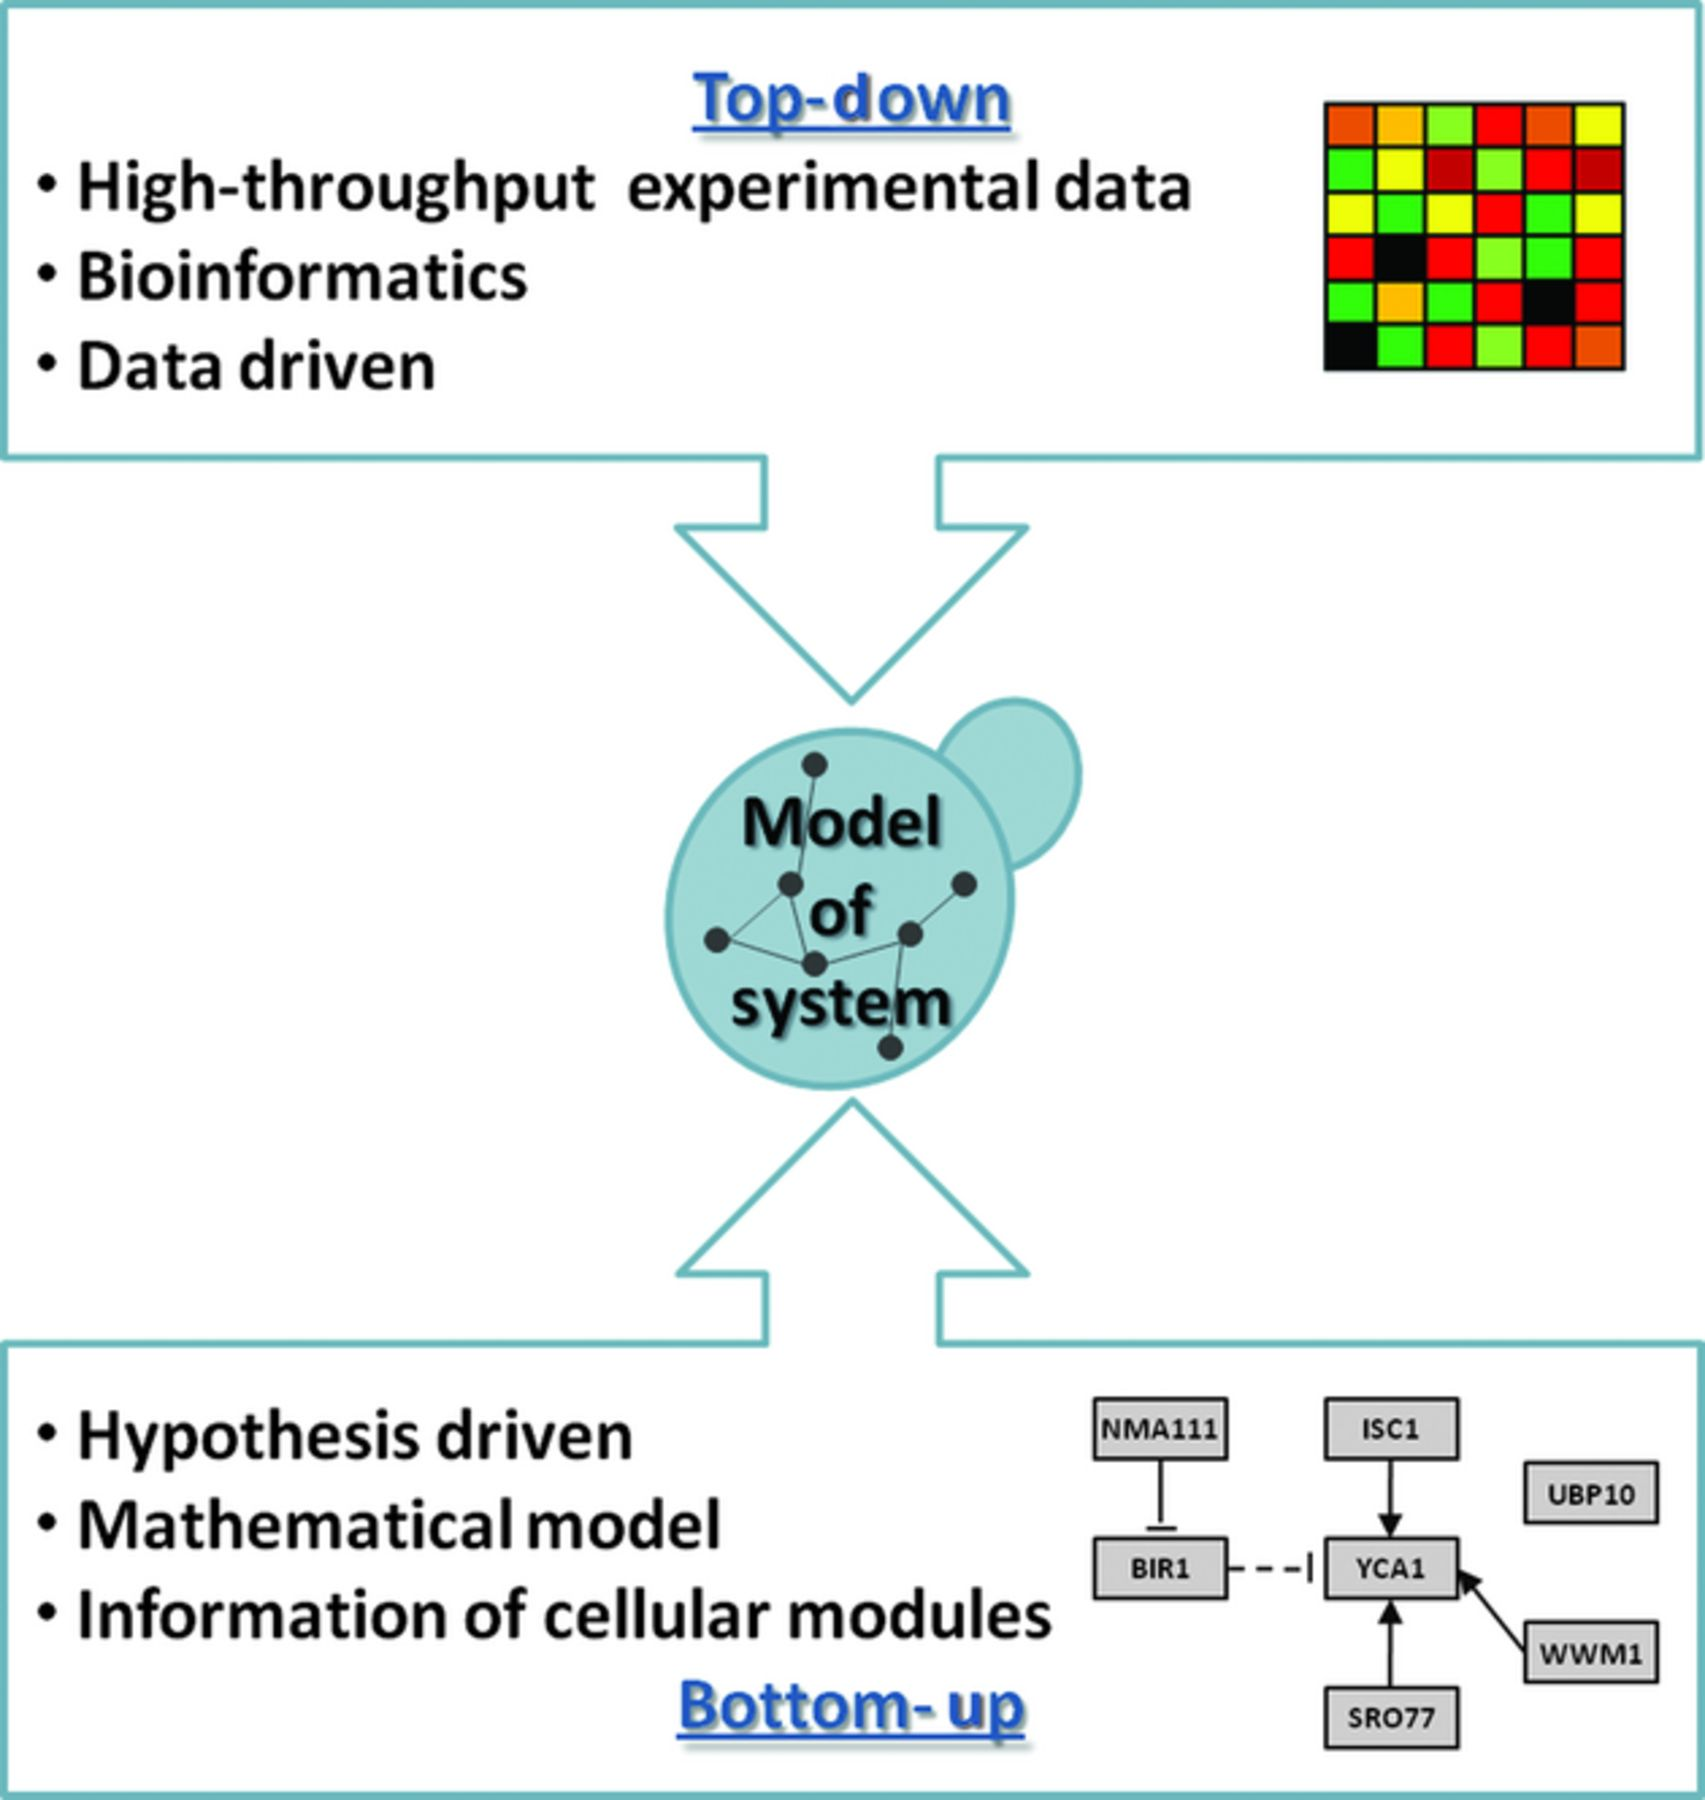
\includegraphics[width=0.6\textwidth]{c1.introduction/sb.tdbu.01.jpg}
  \end{figure}
\end{frame}

\begin{frame}
  \frametitle{概论 | 系统生物学 | 方法 | 整合与干涉 | 整合策略}
  \begin{itemize}
    \item 选用简单的系统,分析尽可能多的构成成分,解释代谢网络和整个系统行为
    \item 研究复杂的系统,采用尽可能多的研究手段
  \end{itemize}
\end{frame}

\begin{frame}
  \frametitle{概论 | 系统生物学 | 方法 | 建模和模拟 | 建模}
  \begin{block}{研究系统的目的}
了解系统各个组成部分之间的关系,预测系统在另一些新情况下的执行情况
  \end{block}
  \pause
  \begin{block}{局限性}
许多系统不具有实际试验的可能性
  \end{block}
  \pause
  \begin{block}{解决办法}
按实际系统建立系统模型,然后利用模型试验研究的结果来推断实际系统的工作
  \end{block}
\end{frame}

\begin{frame}
  \frametitle{概论 | 系统生物学 | 方法 | 建模和模拟 | 建模}
  \begin{figure}
    \centering
    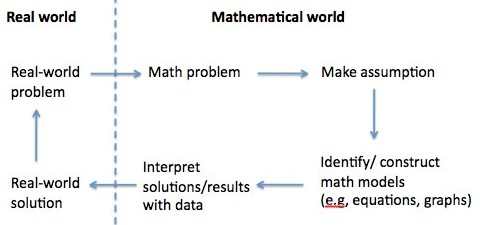
\includegraphics[width=0.9\textwidth]{c1.introduction/sb.model.01.jpg}
  \end{figure}
\end{frame}

\begin{frame}
  \frametitle{概论 | 系统生物学 | 方法 | 建模和模拟 | 模拟}
  \begin{block}{系统模拟}
系统模拟又称为系统仿真,是根据被研究的真实系统的模型,利用计算机进行实验研究的一种方法,它通过模型在计算机上的运行来对模型进行检验和修正,使模型不断趋于完美的进程。  
  \end{block}
  \pause
  \begin{block}{解决两个问题}
    \begin{itemize}
      \item 提供计算机能接受的仿真模型
      \item 提供在计算机上运行计算和进行仿真研究的方法
    \end{itemize}
  \end{block}
  \pause
  \begin{block}{包括三个要素}
      系统、模型、计算机
  \end{block}
  \pause
  \begin{block}{三个基本活动}
     系统模型建立、仿真模型建立、仿真实验
  \end{block}
\end{frame}

\begin{frame}
  \frametitle{概论 | 系统生物学 | 方法 | 建模和模拟 | 模拟}
  \begin{figure}
    \centering
    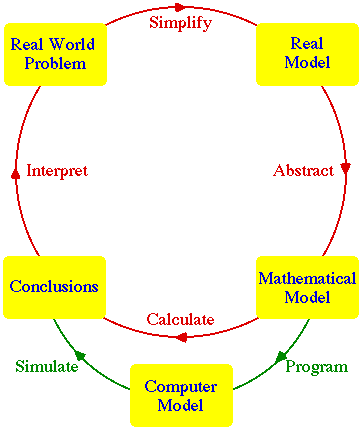
\includegraphics[width=0.55\textwidth]{c1.introduction/sb.simulation.01.png}
  \end{figure}
\end{frame}

\begin{frame}
  \frametitle{概论 | 系统生物学 | 方法 | 建模和模拟 | 模拟}
  \begin{block}{优势}
    \begin{itemize}
      \item 可以求解许多复杂而无法用数学手段解析求解的问题
      \item 可以预测或再现系统的运动规律或运动过程
      \item 可以对无法直接进行实验的系统进行仿真实验研究
    \end{itemize}
  \end{block}
  \pause
  \begin{block}{缺陷}
    \begin{itemize}
      \item 忽略系统的次要因素及不可检测变量
      \item 实际系统的简化近似模型
    \end{itemize}
  \end{block}
\end{frame}

\subsection{应用前景}
\begin{frame}
  \frametitle{概论 | 系统生物学 | 应用}
  \begin{figure}
    \centering
    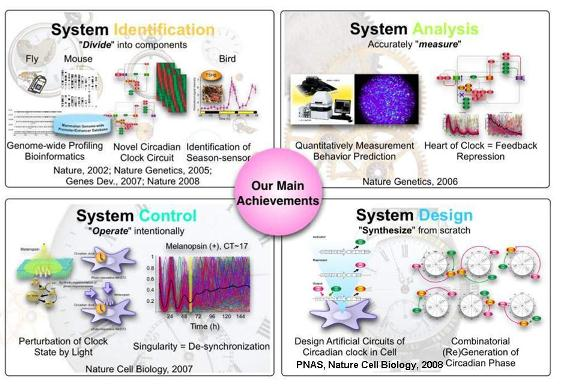
\includegraphics[width=0.9\textwidth]{c1.introduction/sb.application.01.jpg}
  \end{figure}
\end{frame}

\begin{frame}
  \frametitle{概论 | 系统生物学 | 应用}
  \begin{figure}
    \centering
    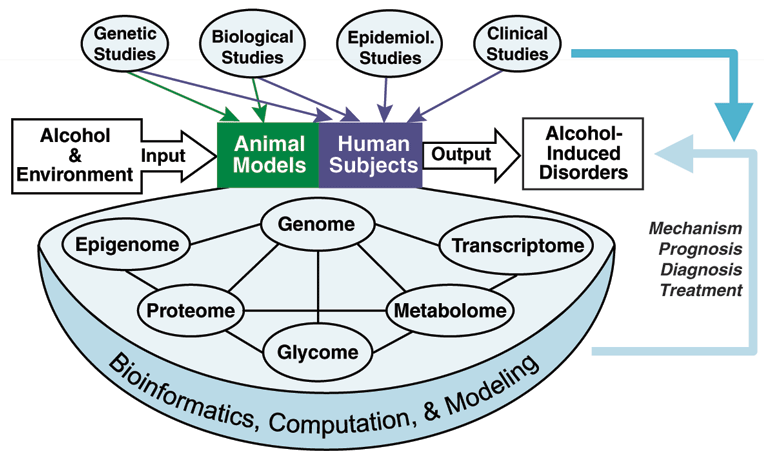
\includegraphics[width=0.9\textwidth]{c1.introduction/sb.application.02.png}
  \end{figure}
\end{frame}

\begin{frame}
  \frametitle{概论 | 系统生物学 | 应用}
  \begin{figure}
    \centering
    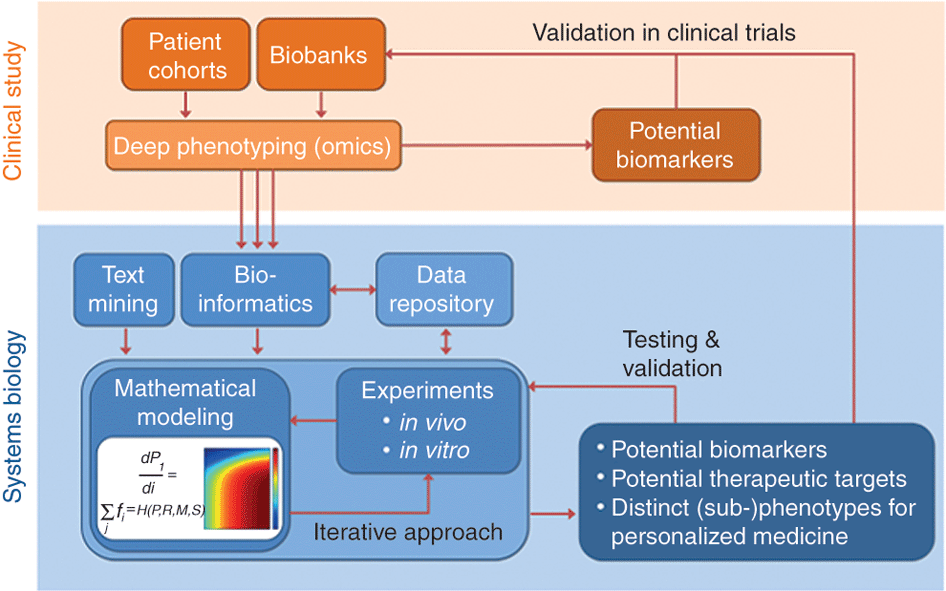
\includegraphics[width=0.9\textwidth]{c1.introduction/sb.application.03.png}
  \end{figure}
\end{frame}

\begin{frame}
  \frametitle{概论 | 系统生物学 | 前景}
  \begin{figure}
    \centering
    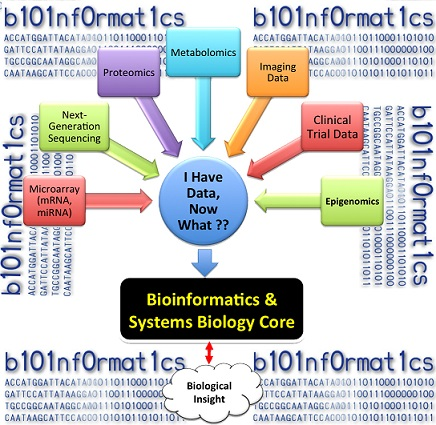
\includegraphics[width=0.6\textwidth]{c1.introduction/sb.future.01.jpg}
  \end{figure}
\end{frame}



\section{回顾与总结}
\subsection{总结}
\begin{frame}
  \frametitle{概论 | 总结}
  \begin{block}{知识点}
    \begin{itemize}
      \item 系统生物学的学科定义。
      \item 系统生物学的研究内容。
      \item 系统生物学的工作流程。
      \item 系统生物学的研究方法。
    \end{itemize}
  \end{block}
  \begin{block}{技能}
    \begin{itemize}
      \item 各种方法论在系统生物学中的应用。
      \item 各种方法论在实际中的应用。
    \end{itemize}
  \end{block}
\end{frame}

\subsection{思考题}
\begin{frame}
  \frametitle{概论 | 思考题}
  \begin{enumerate}
    \item 根据自己的理解说明什么是系统生物学。
    \item 描述系统生物学的研究内容和基本工作流程。
    \item 解释系统生物学研究方法中的“自上而下”和“自下而上”。
  \end{enumerate}
\end{frame}

\begin{frame}
  \frametitle{下节预告}
  \begin{itemize}
    \item 回顾人类基因组计划。
    \item 描述Sanger测序法的基本原理。
    \item 总结生物信息学中常见的数据格式。
  \end{itemize}
\end{frame}




\section*{Acknowledgements}
\begin{frame}
  \frametitle{Powered by}
  \begin{center}
    
\includegraphics[width=9cm]{power.png}
  \end{center}
\end{frame}

\end{document}

